% Enable warnings about problematic code
\RequirePackage[l2tabu, orthodox]{nag}

\PassOptionsToPackage{utf8}{inputenc}
\PassOptionsToPackage{T1}{fontenc}
\PassOptionsToPackage{ngerman, american}{babel}

\title{Computing Language Model Arg-Max-Queries Using Top-\emph{k} Joining Techniques}
\author{Lukas Schmelzeisen}
\date{\today}

\documentclass[m,bachelor,classicthesis,classicthesistitle]{thesis}

\authormail{lukas@uni-koblenz.de}
\degreecourse{Informatik}
\firstreviewer{Prof.~Dr.~Steffen Staab}
\firstreviewerinfo{Institute for Web Science and Technologies}
\secondreviewer{Ren{\'e} Pickhardt}
\secondreviewerinfo{Institute for Web Science and Technologies}

\usepackage{pdflscape}
\usepackage{tikz}

% TODO
\usepackage{paralist}
\newcommand{\inlinecode}[1]{\lstinline[columns=fixed]{#1}}

\addbibresource{bibliography.bib}

% Editorial Commands ===========================================================
% TODO: remove before relase

\usepackage[
  linecolor = Maroon,
  bordercolor = Maroon,
  backgroundcolor = White
]{todonotes}

\definecolor{draft}{rgb}{0.5, 0.5, 0.5}
\newenvironment*{draft}{
  \color{draft}
}{
}

\newcommand*\Lukas[2][]{
  \todo[linecolor = Cyan, bordercolor = Cyan, #1]{Lukas: #2}
}
\newcommand*\Rene[2][]{
  \todo[linecolor = Blue, bordercolor = Blue, #1]{Rene: #2}
}

\newcommand{\noref}{\textcolor{RoyalBlue}{\footnotesize[Citation needed]}}
\newcommand{\mbref}[1]{\textcolor{RoyalBlue}{\footnotesize[Citation: #1?]}}

% ==============================================================================

\begin{document}
\frenchspacing
\raggedbottom

% Frontmatter ==================================================================

\pagestyle{scrplain}
\pagenumbering{roman}

\selectlanguage{ngerman}
\maketitle
\selectlanguage{american}

\cleardoublepage
\pdfbookmark[1]{Abstract}{Abstract}
\begin{abstractpage}
  \begin{abstract}
    Next word prediction is the task of guessing the next word a user intends to
    type from the words they have already entered.
    Traditionally, this problem is solved by calculating an argmax of language
    model probabilities for all words in a vocabulary.
    However, this approach is slow and becomes linearly worse with
    increasing vocabulary size.
    This thesis proposes two independent optimizations.
    First, a novel approach is presented that allows for performing part of the
    probability calculation in a precomputation step.
    Second, it is shown how to apply top-k joining techniques to word
    prediction to avoid iterating all words in the vocabulary.
    Using both optimizations sub-millisecond next word prediction time is
    achieved.
  \end{abstract}

  \selectlanguage{ngerman}
  \begin{abstract}
    Next-Word-Prediction ist die Problemstellung das nächste Wort vorherzusagen,
    welches ein Benutzer zu tippen beabsichtigt, mit Hilfe der Kenntnis, welche
    Wörter bereits eingetippt wurden.
    Für gewöhnlich wird dieses Problem mit Hilfe eines Argmax über
    Sprachmodellwahrscheinlichkeiten aller Wörter eines Vokabulars gelöst.
    Diese Ansatz ist jedoch langsam und wird mit wachsender Vokabulargröße
    linear schlechter.
    Diese Arbeit schlägt zwei unabhängige Optimierungen vor.
    Zum einen wird ein neuartiger Ansatz vorgestellt, der es erlaubt einen Teil
    der Wahrscheinlichkeitsberechnung in einem Vorberechnungsschritt
    auszuführen.
    Zum anderen wird gezeigt wie Top-k-Joining-Verfahren zur Berechnung der
    Wortvorhersage eingesetzt werden können.
    Dies ermöglicht es, die Iteration über aller Wörter des Vokabulars zu
    vermeiden.
    Unter Einsatz beider Optimierungen wurden Vorhersagezeiten unter einer
    Millisekunde erzielt.
  \end{abstract}
  \selectlanguage{american}
\end{abstractpage}



\clearpage
\todo[inline]{License!}
\todo[inline,caption={Discussion with Ren{\'e}}]{
  Discussion with Ren{\'e}:
  \begin{itemize}
    \item Is ``we'' ok, when single author?
    \item Are chapters ok?
    \item Capitalize in document reference?
    \item Citation style?
    \item Conditions after Equations ok as in \cref{ch:review-lm}?
    \item Scope ok? Not too long or short?
    \item Terminology: Probability event? Interpolation weight/argument?
  \end{itemize}
}
\todo[inline]{Use standalone documents for figures.}
\todo[inline]{Use etoolbox for ifthenelse in class.}
\todo[inline]{Kill warnings.}
\todo[inline]{Rewrite math package. Use left/right braces for set.}

\cleardoublepage
\pdfbookmark[1]{\contentsname}{toc}
\tableofcontents

% Mainmatter ===================================================================

\cleardoublepage
\pagenumbering{arabic}
\pagestyle{scrheadings}

\chapter{Introduction}

\begin{draft}
Introduction pargraph: We solve noisy channel argmax with Top-$k$ joining
techniques.
\end{draft}

The \emph{noisy channel model} is a commonly applied concept in natural language
processing.
As first described by \textcite{Shannon1948}, it consists of a transmitter, who
tries to pass a message over a channel to a receiver.
The channel is called noisy, because it may distort the message in any way.
The task is then to reconstruct the original message, from the recieved
distorted one.

This metaphor has many applications, such as spelling correction
\parencite{JurafskyMartin2009,Manning2008,Kernighan1990,Mays1991},
%          \------------- non-word-errors ------------/    \- real-word-erros
part-of-speech-tagging \parencite{Church1988}, machine translation
\parencite{Brown1990}, speech recognition or text compression.
\todo{Find newer citations. Maybe from \textcite{Bickel2005}}
% JurafskyMartin2009: Chapter 5: Spelling Correction
%                     Chapter 9: Speech Recognition!

Formalized, this task of the noisy channel model is to find the dispatched
message~$m$, which is the sequence of words $s = w_1^n = w_1 \ldots w_n$ in a
langauge~$\Language$ that is most likely to be the source of the received
distorted observation~$o$:
\begin{align}
  \label{eq:noisychannel}
  m &= \Argmax_{s \in \Language} \Prob{s}{o} \\
  \intertext{Using Bayes' theorem one can rewrite this to:}
  \label{eq:noisychannelbayes}
  \begin{split}
    m &= \Argmax_{s \in \Language} \frac{\Prob{o}{s} \cdot \Prob{s}}{\Prob{o}} \\
      &= \Argmax_{s \in \Language} \Prob{o}{s} \cdot \Prob{s}
  \end{split}
\end{align}
With the observation likelihood~$\Prob{o}{s}$ and the prior
probability~$\Prob{s}$.
Omitting the denominator~$\Prob{o}$ is valid because it is a constant that does
not depend on the argument~$s$.
Most commonly the observation likelihood is some domain specific probability
distribution $\Prob[\text{Domain}]{o}{s}$, for the prior probability
\emph{statistical language models} are used.
They assign a probability $\Prob[\text{LM}]{s}$ to a sequence of words
$s = w_1^n = w_1 \ldots w_n$ by means of a probability distribution, created
through statistical analysis of text corpora.
Thus the noisy channel model is a natural combintion of domain knowledge with
language information.

\Lukas{It is possible to omit this paragraph, but I think it provides
clarification.}
For example, to translate French into English, \textcite{Brown1990} defined a
probability distribution $\Prob[\text{Translate}]{e}{f}$, that would give the
probability for each English sentence $e$ to be the result of translating
the French sentence $f$ into English.
To obtain the most likely translation, the $e$ that maximizes that probability
has to be found.
With applying Bayes' theorem they combine their distribution with language
models and arrive at
$\Argmax_{e} \Prob[\text{Translate}]{f}{e} \cdot \Prob[\text{LM}]{e}$, which is
just \cref{eq:noisychannelbayes}.

A major problem in creating statistical language models from text corpora, is
that even for very large corpora, most possible word sequences in a language
will not be observed in training \noref.
A common approximation are \emph{$n$-gram models}, in which it is assumed that
the probability of a word only depdens on the $n\!-\!1$~previous words, thus
only sequences of length $n$ have to be considered.

State-of-the-art language models use $n$-grams with $n$ as large as $5$
\mbref{JurafskyMartin2009,Goodman2001}.
\begin{draft}
\Cref{eq:noisychannel} is hard to calculate for such large $n$.
So we want to optimize that.
\end{draft}

\begin{draft}
We try to use top-$k$ joining.

We are interested in \emph{next word prediction} $\NWP$ and
\emph{next keystroke savings} $\NKSS$.

So we have to map our problem on the realm of top-$k$ joining.

We apply that technique.

May be good because we do not have to prune, and pruning might be bad
\parencite{Stolcke2000,Chelba2013,Chelba2010,Siivola2007}.

Most non-trivial top-\emph{k} joining algorithms require a monotone scoring
function, some further improvements can be made if using a linear scoring
function~\parencite{Ilyas2008}.
\end{draft}

\begin{draft}
Introduction to next word predition.
\todo{Read \textcite{Bickel2005} for info.}
\end{draft}

\begin{draft}
Overview of following chapters.
\end{draft}

\chapter{Related Work}
\label{ch:relatedwork}

\begin{draft}
\begin{displayquote}[\textcite{JurafskyMartin2009}]
Because in practice most implementations of Viterbi use beam
search, some of the literature uses the term beam search or time-synchronous beam
search instead of Viterbi.
\end{displayquote}
\end{draft}

% ------------------------------------------------------------------------------
\section{Noisy Channel Queries}

The established way to solve noisy channel type queries is to use
\emph{Viterbi-} or \emph{beam-search-algorithms}
\parencite{JurafskyMartin2009,Bickel2005}.
These algorithms are based on following most promising looking paths and
pruning the search space with some heuristic.
Trough this pruning, remarkable runtime performance can be achieved, however it
has other undesirable effects, for instance these algorithms are not guaranteed
to always find (optimal) solutions \parencite{Bickel2005}.

This thesis' approach using top-$k$ joining does not have these drawbacks, it
will always find the best solution(s).

% ------------------------------------------------------------------------------
\section{State-of-the-art Language Models}

The currently most commonly used \parencite{JurafskyMartin2009,Chelba2013}
technique for estimating language models is \emph{Modified Kneser-Ney Smoothing}
by \textcite{ChenGoodman1996,ChenGoodman1998,ChenGoodman1999}, based on
\emph{Kneser-Ney Smoothing} by \textcite{KneserNey1995}.
\textcite{BilmesKirchhoff2003} introduced the concept of a \emph{generalized
parallel backoff}, which very recently \textcite{Pickhardt2014} used to provide
a generalization of Modified Kneser-Ney Smoothing, the \emph{Generalized
Language Model}.

\begin{draft}
Justify selection of MKN and GLM over recently popular LMs from
\textcite{Chelba2013}.
\end{draft}

An in-depth summary of Modified Kneser-Ney Smoothing and the Generalized
Language Model is given in \cref{ch:review}.

We will then express these language models as weighted sums of their occurrence
counts in \cref{ch:weightedsum}.
To the authors knowledge, there is no other work on expressing language models
as weighted sums.
However, \textcite{JelinekMercer1980} already experimented with trying to learn
weighted sum parameters automatically for language modeling.

\begin{draft}
Mention \emph{Nerual Network Language Models} \parencite{Bengio2003,Mikolov2012}
(do we not use them because they can not be represented as weighted sums?), as
they seem to be in favor of academic research recently.
\end{draft}

% ------------------------------------------------------------------------------
\section{Top-\emph{k} Joining Techniques}

\textcite{Ilyas2008} survey a wide range of different top-$k$ processing
techniques.
One way to distinguish top-$k$ techniques is data access.
Nearly all algorithms necessitate some form of \emph{sorted access} to data
sources.
Some techniques additionally require \emph{random access}.

Among others, two fundamental algorithms were established by
\textcite{Fagin2001}: the \emph{threshold algorithm} (sorted and random access)
and the \emph{no-random-access algorithm} (only sorted access).
The implementation for these two algorithms will be described in
\cref{ch:topkjoin}, and we will evaluate them in \cref{ch:evaluation}.

\begin{draft}
Mention instance optimiallity, and else Fagin proved.
\end{draft}


\begin{draft}
Mention \textcite{Guentzer2000} and \textcite{Guentzer2001} improvements to TA
and NRA.
\end{draft}

\begin{draft}
Mention other more optimized techniques such as onion indices or J* or
Rank-Join.
How do I explain these can not be used in this chapter?
\end{draft}

\chapter{Review of Considered Language Models}
\label{ch:review-lm}

This chapter will recall language modeling techniques considered in this work,
and introduce the used notation (\cref{sec:review-notation}).
Namely, \emph{Modified Kneser-Ney Smoothing} (\cref{sec:review-lm-mkn})
and the \emph{Generalized Language Model} (\cref{sec:review-lm-glm})
are described.

\todo[inline, caption = {Citations in Review}]{
  How do I declare citations for this section?
  \begin{itemize}
    \item Do I cite Rene or ChenGoodman?
    \item Do I cite once or on every definition?
    \item Some stuff is not published anywhere else yet. (For example new skip
      notation or new glm notation)
  \end{itemize}
}

% ------------------------------------------------------------------------------
\section{Notation: Counts and Skips}
\label{sec:review-notation}

Let $\Count(w_1^n)$ denote the frequency count of a sequence's
$w_1^n = w_1 \ldots w_n$ occurence in training data.

Let $\Skp$ be a wildcard (called \emph{``skip''}), that can take the place
of any word at its location.
Thus, for example $\Count(\Skp w_1^n)$ is the frequency count of sequences
in training data who start with any word $x \in \Sigma$ and were the remaining
words are $w_1^n$:
\begin{equation}
  \Count(\Skp w_1^n) = \sum_{x \in \Sigma} \Count(x \: w_1^n)
\end{equation}
Where $\Sigma$ is the set of all words in a language
$\Language \subseteq \Sigma^{*}$.
It is easy to extend this definition to sequences with multiple skips:
\begin{equation}
  \Count(w_1 \Skp \Skp w_2) = \sum_{x, y \in \Sigma} \Count(w_1 \: x \: y \: w_2)
\end{equation}

\todo[inline]{Do we mention the difference of $\Count(\Skp w_1^n)$ to $\Count(w_1^n)$
in absence of Beginning of Sentence tags?}

Additionally we define \emph{continuation} counts $\ContCount_k(\DummyArg)$ as
the number of sequences from the training data that occur exactly $k$ times and
can be constructed by replacing $\WSkp$ (called \emph{``continuation skip''})
with any word $x \in \Sigma$.
For example $\ContCountII(\WSkp w_1^n)$ denotes the number of words that can
precede $w_1^n$ in training data, and occur exactly $2$ times:
\begin{equation}
  \ContCountII(\WSkp w_1^n) =
    \Cardinality{\left\{ x \in \Sigma \,\middle|\, \Count(x \: w_1^n) = 2 \right\}}
\end{equation}
Further let $\ContCount_{k+}(\DummyArg)$ count sequences that occur $k$ or more
times:
\begin{equation}
  \ContCountIp(\WSkp w_1^n) =
    \Cardinality{\left\{ x \in \Sigma \,\middle|\, \Count(x \: w_1^n) \geq 1 \right\}}
\end{equation}

In continuation counts regular skips and continuation skips can be mixed, for
example:
\todo{Check this equation!}
\begin{equation}
  \ContCountIp(\WSkp w \Skp \WSkp) =
    \Cardinality{\left\{ x, y \in \Sigma \,\middle|\, c(x \: w \Skp y) \geq 1 \right\}}
\end{equation}

To make a clear distinction between ``normal'' counts $\Count(\DummyArg)$ and
continuation counts $\ContCount_{\DummyIndex}(\DummyArg)$, we
sometimes call the former \emph{absolute} counts.

% ------------------------------------------------------------------------------
\section{Modified Kneser-Ney Smoothing}
\label{sec:review-lm-mkn}

\begin{draft}
Modified Kneser-Ney smoothed language models are computed by interpolating
between higher and lower order $n$-gram language models.
The highest order distribution is interpolated with lower order distirbutions
as follows:
\todo{(Copied from Rene)}
\end{draft}
\begin{equation}
  \label{eq:mkn-high}
  \ProbMKN{w_n}{w_1^{n-1}} =
    \frac{\DiscountedCount(w_1^n) + \gamma(w_1^{n-1}) \ProbMKN*{w_n}{w_1^{n-2}}}
         {\Count(w_1^{n-1} \Skp)} \\
\end{equation}
With the \emph{discounted} count
${\DiscountedCount(w_1^n) = \max\Set{\Count(w_1^n) - \Discount(\Count(w_1^n)), 0}}$.

The exact definitions of $D(\DummyArg)$ and $\gamma(w_1^{n-1})$ are not
important in our context, however for the sake of completeness they are given
in \cref{sec:discounts-interpolation-weights}.

Naturally \cref{eq:mkn-high} is only defined if the denominator
${\Count(w_1^{n-1} \Skp) > 0}$, that is if the history $w_1^{n-1} \Skp$ was seen
in training.
If $w_1^{n-1} \Skp$ was not seen, we perform a so called \emph{``back-off''}
and set:
\begin{align}
  \label{eq:mkn-backoff}
  \ProbMKN{w_n}{w_1^{n-1}} = \ProbMKN{w_n}{w_1^{n-2}}
      & & \Condition{\Count(w_1^{n-1} \Skp) = 0}
\end{align}
It is common to perform multiple back-offs until the history was actually seen.
\todo{This should actually not be true, because we increase n-gram length for
first lower order. How do we handle this in current implementation?}

\begin{draft}
Essentially, interpolation with a lower order model corresponds to leaving out
the first word in the considered sequence.
\todo{(Copied from Rene)}
\end{draft}
Lower order models are computed differently, and in turn interpolated with
further lower orders:
\begin{equation}
  \label{eq:mkn-low}
  \ProbMKN*{w_n}{w_1^{n-1}} =
    \frac{\DiscountedCount*(\WSkp w_1^n) + \gamma(w_1^{n-1}) \ProbMKN*{w_n}{w_1^{n-2}}}
         {\ContCountIp(\WSkp w_1^{n-1} \WSkp)} \\
\end{equation}
With the \emph{discounted} continuation count
${\DiscountedCount*(\WSkp w_1^n) = \max\Set{ \ContCountIp(\WSkp w_1^n) - \Discount(\Count(w_1^n)), 0 }}$.
Backing-off to compute lower orders is never necessary, because
if history $w_1^{n-1}$ was seen, $w_1^{n-2}$ was seen as well.

The lowest order (the probability of a single word) can not be further
interpolated and we use the relative continuation frequency of that word.
Similarly if we only want to compute the probability of a single word on the
highest order, we compute it as the relative frequency of that word:
\begin{subequations}
  \label{eq:mkn-lowest}
  \begin{align}
    \ProbMKN {w} &= \frac{\Count(w)}{\Count(\Skp)} \\
    \ProbMKN*{w} &= \frac{\ContCountIp(\WSkp w)}{\ContCountIp(\WSkp \WSkp)}
  \end{align}
\end{subequations}

% ------------------------------------------------------------------------------
\section{Generalized Language Model}
\label{sec:review-lm-glm}

The Generalized Language Model is a natural extension to Modified Kneser-Ney
Smoothing.
It is again based on interpolation, though it differs in the way lower order
models are interpolated.
The highest order is computed as:
\begin{equation}
  \label{eq:glm-high}
  \ProbGLM{w_n}{w_1^{n-1}} =
    \frac{\DiscountedCount(w_1^n) + \frac{\gamma(w_1^{n-1})}{\#_\partial(w_1^{n-1})}
                                    \sum_{j=1}^{\#_\partial(w_1^{n-1})} \ProbGLM*{w_n}{\partial_j w_1^{n-1}}}
         {\Count(w_1^{n-1} \Skp)}
\end{equation}
Auxiliary definitions $\DiscountedCount, \DiscountedCount*, \gamma$ are the same
as for Modified Kneser-Ney Smoothing and given in \cref{sec:review-lm-mkn}.

The skip operator $\partial_j w_1^{n-1}$ can be any mapping that relates
$w_1^{n-1}$ to exactly $\#_\partial(w_1^{n-1})$ many derived sequences.
It is easy to see that for $\#_\partial(w_1^{n-1}) = 1$ and
$\partial_1 w_1^{n-1} = w_2^{n-1}$ \cref{eq:glm-high} is an
instantiation of \cref{eq:mkn-high} (Modified Kneser-Ney Smoothing), and thus
a true generalization.

In practice only one definition for $\partial$ is used though.
That is $\#_\partial(w_1^{n-1})$ is set to the number of non-skip words in
$w_1^{n-1}$ and $\partial_j(w_1^{n-1})$ replaces the $j$th non-skip word with
a skip.
For instance: $\partial_2(w_1^3) = w_1 \Skp w_3$.

Again as with Modified Kneser-Ney Smoothing, \cref{eq:glm-high} is not
defined if $w_1^{n-1}$ is unseen and thus our denominator would be zero.
The back-off step is then performed as:
\begin{equation}
  \label{eq:glm-backoff}
  \begin{split}
    \ProbGLM{w_n}{w_1^{n-1}} = \frac{1}{\#_\partial(w_1^{n-1})}
                               \sum_{j=1}^{\#_\partial(w_1^{n-1})} \ProbGLM{w_n}{\partial_j w_1^{n-1}} \\
      \hfill \Condition{\Count(w_1^{n-1} \Skp) = 0}
  \end{split}
\end{equation}

Subsequently lower order models are computed as:
\begin{equation}
  \label{eq:glm-low}
  \ProbGLM*{w_n}{w_1^{n-1}} =
    \frac{\DiscountedCount*(\WSkp w_1^n) + \frac{\gamma(w_1^{n-1})}{\#_\partial(w_1^{n-1})}
                                     \sum_{j=1}^{\#_\partial(w_1^{n-1})} \ProbGLM*{w_n}{\partial_j w_1^{n-1}}}
         {\ContCountIp(\WSkp w_1^{n-1} \WSkp)}
\end{equation}
\todo[inline]{Replace \Skp with \WSkp in $\ContCountIp$ in GLM?}
\todo[inline]{\WSkp at end of $\ContCountIp$ correct?}

The case of the lowest order occurs when $\#_\partial(w_1^{n-1}) = 0$ and is
handled similarly to Modified Kneser-Ney Smoothing.
In practice this is the case when $w_1^{n-1}$ only consists of skips.
\begin{subequations}
  \label{eq:glm-lowest}
  \begin{align}
    \ProbGLM {w_n}{w_1^{n-1}} &= \frac{\Count(w_1^n)}{\Count(w_1^{n-1} \Skp)}
      & \Condition{\#_\partial(w_1^{n-1}) = 0} \\
    \ProbMKN*{w_n}{w_1^{n-1}} &= \frac{\ContCountIp(\WSkp w_1^n)}{\ContCountIp(\WSkp w_1^{n-1} \WSkp)}
      & \Condition{\#_\partial(w_1^{n-1}) = 0}
  \end{align}
\end{subequations}

% ------------------------------------------------------------------------------
\section{Discounting and Interpolation Weights}
\label{sec:discounts-interpolation-weights}

\begin{draft}
Explain Discounting and Smoothing.
\end{draft}

\begin{draft}
\begin{equation}
  \Discount(c) =
    \begin{dcases*}
      0      & if $c = 0$ \\
      D_1    & if $c = 1$ \\
      D_2    & if $c = 2$ \\
      D_{3+} & if $c \geq 3$
    \end{dcases*}
\end{equation}

\begin{subequations}
  \begin{align}
    D_1    &= 1 - 2 Y \frac{n_2}{n_1} \\
    D_2    &= 2 - 3 Y \frac{n_3}{n_2} \\
    D_{3+} &= 3 - 4 Y \frac{n_4}{n_3}
  \end{align}
\end{subequations}

\begin{equation}
  Y = \frac{n_1}{n_1 + n_2}
\end{equation}

\begin{equation}
  \gamma(w_1^{n-1}) =   D_1    \ContCountI    (w_1^{n-1} \WSkp)
                      + D_2    \ContCountII   (w_1^{n-1} \WSkp)
                      + D_{3+} \ContCountIIIp (w_1^{n-1} \WSkp)
\end{equation}
\end{draft}

\chapter{Formulating Language Models as Weighted Sums}
\label{ch:weightedsum}

In this chapter we will present a novel way to represent the probabilities
$\ProbMKN{w_n}{w_1^{n-1}}$ and $\ProbGLM{w_n}{w_1^{n-1}}$ as weighted sums of
terms depending on $w_n$, for a fixed history $h = w_1^{n-1}$ and an  arbitrary
probability event $w = w_n$.
In other words we will express the formulas given in \cref{ch:review} as
equations of the following form:
\begin{equation}
  \label{eq:weightedsum}
  \Prob{w}{h} = \sum_{i = 1}^{N} \SumWeight_i^h \cdot \SumArg_i^h(w)
\end{equation}
Where $N$ is the number of interpolation factors dependent on the choice of
language model.

To the author's knowledge, there is no other work on expressing existing
language models as weighted sums.
However, \textcite{JelinekMercer1980} already experimented with learning
weighted sum parameters automatically for language modeling.

Being able to accurately represent probabilities in a form like this is highly
beneficial for word prediction.
As we can see in \cref{eq:prefixquery} the computation for next word prediction
is based on calculating multiple probabilities $\Prob{w}{h}$ with a fixed
history $h$ but varying arguments $w$.
As has been specified in \cref{ch:review}, probability calculation is based on
complex recursive formulas.
Using our weighted sum representation this computation can be sped up by
a huge factor, since the computation of the sum weights $\SumWeight^h_i$ can
be performed once beforehand.
For each final probability we then only have to perform the $N$ remaining
lookups $\SumArg^h_i(w)$ that actually depend on $w$.

Another handy benefit is that by this representation we have all terms that
change with $w$ explicitly available, which is a prerequisite for top-$k$
joining and will be explained in \cref{ch:topkjoin}.
Last, our algorithms for calculating sum weights turn out to be performing
faster than the direct recursive implementations, which we measure in
\cref{sec:evaluation-weightedsum}.

We will now present the basic idea of how to transform a probability
$\Prob{w_n}{w_1^{n-1}}$ into a weighted sum that applies to both Modified
Kneser-Ney Smoothing and the Generalized Language Model:

Note that in all \cref{eq:mkn-high,eq:mkn-low,eq:glm-high,eq:glm-low} the
probability event $w_n$ only appears in the nominator of fractions, specifically
in the argument terms of $\DiscountedCount$ or $\DiscountedCount*$.
Additionally $w_n$ occurs as arguments for $\Count$ and $\ContCountIp$ in the
lowest order \cref{eq:mkn-lowest,eq:glm-lowest}.
Our general idea is thus, to first expand recursive calls to
$\Prob(\DummyArg)$ or $\Prob*(\DummyArg)$, and second to factor
out the terms that do not depend on $w_n$ by the distributive property.

\Cref{sec:weightedsum-mkn} explains our approach for Modified Kneser-Ney
Smoothing, while \cref{sec:weightedsum-glm} concerns itself with the Generalized
Language Model.


% ------------------------------------------------------------------------------
\clearpage
\section{Modified Kneser-Ney Smoothing}
\label{sec:weightedsum-mkn}

Modified Kneser-Ney Smoothed probabilities $\ProbMKN{w}{h}$ are calculated as
follows (\cref{sec:review-lm-mkn}):
\begin{enumerate}
  \item Backing-off: Leave out words at the beginning of the history $h$, until
    $h \Skp$ is seen for the first time (\cref{eq:mkn-backoff}).
  \item Highest order: Look up frequency counts $\DiscountedCount(h \: w)$ and
    $\Count(h \Skp)$ (\cref{eq:mkn-high}) and shorten the history by one word.
  \item Lower orders: Look up continuation counts $\DiscountedCount*(\WSkp h \: w)$
    and $\ContCountIp(\WSkp h \WSkp)$ (\cref{eq:mkn-low}) and shorten the
    history further until it is empty.
  \item Lowest order: Look up continuation counts $\ContCountIp(\WSkp w)$ and
    $\ContCountIp(\WSkp \WSkp)$ (\cref{eq:mkn-lowest}).
\end{enumerate}

\newcommand{\ProbMKNcab}[1]
  {\frac{\DiscountedCount(w_1 w_2 w_3) + \gamma(w_1 w_2) #1}{\Count(w_1 w_2 \Skp)}}
\newcommand{\ProbMKNcb}[1]
  {\frac{\DiscountedCount*(\WSkp w_2 w_3) + \gamma(w_2) #1}{\ContCountIp(\WSkp w_2 \WSkp)}}
\newcommand{\ProbMKNc}
  {\frac{\ContCountIp(\WSkp w_3)}{\ContCountIp(\WSkp \WSkp)}}

% - - - - - - - - - - - - - - - - - - - - - - - - - - - - - - - - - - - - - - -
\subsection{Example}

As an example we will give the full formula expansion necessary to calculate
$\ProbMKN{w_3}{w_1 w_2}$ for any sequence $w_1 w_2 w_3$, assuming sequence
$w_1 w_2 \Skp$ was seen:
\begin{subequations}
  \begin{align}
    \ProbMKN {w_3}{w_1 w_2} &= \ProbMKNcab{\ProbMKN*{w_3}{w_2}} \\
    \ProbMKN*{w_3}{w_2}     &= \ProbMKNcb{\ProbMKN*{w_3}} \\
    \ProbMKN*{w_3}          &= \ProbMKNc
  \end{align}
\end{subequations}
Inserting the lower orders results in:
\begin{equation}
  \ProbMKN {w_3}{w_1 w_2} = \ProbMKNcab{\ProbMKNcb{\ProbMKNc}}
\end{equation}
By using the distributive property we obtain:
\begin{align}
  \label{eq:probmknexpansion-final}
  \hspace{-2.5em}\ProbMKN {w_3}{w_1 w_2} = {}
    & & \DiscountedCount (w_1 w_2 w_3)   & \cdot\ \frac{1}{\Count(w_1 w_2 \Skp)} \\
    &+& \DiscountedCount*(\WSkp w_2 w_3) & \cdot\ \frac{\gamma(w_1 w_2)}{\Count(w_1 w_2 \Skp) \ContCountIp(\WSkp w_2 \WSkp)} \nonumber \\
    &+& \ContCountIp(\WSkp w_3)          & \cdot\ \frac{\gamma(w_1 w_2) \: \gamma(w_2)}{\Count(w_1 w_2 \Skp) \ContCountIp(\WSkp w_2 \WSkp) \ContCountIp(\WSkp \WSkp)} \nonumber
\end{align}

In the final equation \cref{eq:probmknexpansion-final} we can clearly identify
the terms that do depend on $w_3$ and the ones that do not.
Note that $w_3$ never occurs on the right side of the multiplication dot.
Per line the left side of the multiplication dot will form the terms
$\SumArg^h_i(w_3)$, while the right side will form the sum weights
$\SumWeight^h_i$.

But note that this is only valid if the sequence $w_1 w_2 w_3$ has been seen in
the training corpus, and thus $\Count(w_1 w_2 w_3) \geq 1$.
If this is not the case, backoff steps have to be performed, and a different
resulting formula is obtained.

% - - - - - - - - - - - - - - - - - - - - - - - - - - - - - - - - - - - - - - -
\subsection{Sum Terms}

All counts except the ones of the lowest order are discounted using
$\DiscountedCount$ and $\DiscountedCount*$ to interpolate that order with the
following by the weight $\gamma(h)$.
This process of interpolating different orders is visualized in
\cref{fig:history-mkn} for the case of a history of length three.
Building similar backoff graphs for other history lengths is straightforward.

\begin{figure}[tb]
  \centering
  \documentclass{standalone}
\usepackage[dvipsnames,svgnames,x11names]{xcolor}
\usepackage{tikz}
\usepackage{../thesismath}
\begin{document}
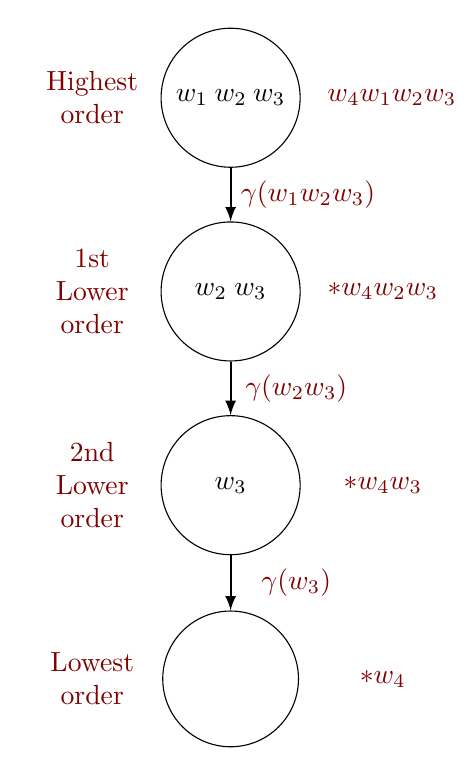
\begin{tikzpicture}
  \tikzset{
    state/.style  = {draw, circle, align = center, text centered, text width = 4.2em},
    invis/.style  = {text width = 4.2em},
    order/.style  = {align = center, text centered, text width = 4em, text = Maroon},
    number/.style = {xshift = 1em, text = Maroon},
  }

  \begin{scope}[node distance = 7em]
    \node [state] (highest)                    {$w_1 \: w_2 \: w_3$};
    \node [state] (lower1)  [below of=highest] {$w_2 \: w_3$};
    \node [state] (lower2)  [below of=lower1]  {$w_3$};
    \node [state] (lowest)  [below of=lower2]  {$\varnothing$};
  \end{scope}

  \begin{scope}[node distance = 5.5em]
    \node [order] [right of=highest] {$\ProbMKN {w_4}{w_1 w_2 w_3}$};
    \node [order] [right of=lower1]  {$\ProbMKN*{w_4}{w_2 w_3}$};
    \node [order] [right of=lower2]  {$\ProbMKN*{w_4}{w_3}$};
    \node [order] [right of=lowest]  {$\ProbMKN*{w_4}$};
  \end{scope}

  \begin{scope}[node distance = 5em]
    \node [order] [left of=highest] {Highest order};
    \node [order] [left of=lower1]  {1st Lower order};
    \node [order] [left of=lower2]  {2nd Lower order};
    \node [order] [left of=lowest]  {Lowest order};
  \end{scope}

  \path[->, >=latex, thick]
    (highest) edge node [right, order] {$\textstyle{\gamma(w_1 w_2 w_3)}$} (lower1)
    (lower1)  edge node [right, order] {$\textstyle{\gamma(w_2 w_3)}$}     (lower2)
    (lower2)  edge node [right, order] {$\textstyle{\gamma(w_3)}$}         (lowest);
\end{tikzpicture}
\end{document}

  \caption{
    The \emph{backoff graphs} shows the interpolation of different orders during
    computation of $\ProbMKN{w_4}{w_1 w_2 w_3}$.
    Centered are the histories for each probability.
    It is assumed that the history $w_1 w_2 w_3$ was seen during training, so
    that no backing-off is necessary.
    Orders are combined with interpolation weights $\gamma(\DummyArg)$.
  }
  \label{fig:history-mkn}
\end{figure}

Each order with a history $h^\prime$ is interpolated with the following order where
the first word of $h^\prime$ is removed.
Thus a total ordering on the histories of the orders can be specified.
In \cref{fig:history-mkn} we have thus assigned each history a number from
$1$~to~$4$.
Let $\DerivedHistory[i]$ denote the history of that graph with number $i$.

The first step in expressing $\ProbMKN{w}{h}$ as a weighted sum is finding the
number $N$ of sum weights.
In the case of Modified Kneser-Ney Smoothing this is exactly the number of
interpolation orders.
Let $\DerivedHistory[s]$ be the first seen history that is the result of
backing-off given history $h$ exactly $s$ times.
The number $N$ of sum weights is then the number of words of that history plus
one for the empty history.
\begin{equation}
  \label{eq:weightedsum-mkn-num}
  N = \NGramLength{\DerivedHistory[s]} + 1
\end{equation}
Where $\NGramLength{w_1^n} = n$ is the length of the $n$-gram $w_1^n$.

The next step is to find the actual terms $\SumArg_i^h(w)$ that shall be
weighted and added.
When looking at the equations that define Modified Kneser-Ney we note the fact
that only the count terms in the numerators depend on the probability event $w$.
Exactly these terms compose our sum arguments:
\begin{equation}
  \SumArg_i^h(w) =
    \begin{dcases*}
      \Count(w)                                             & if $N = 1$ \\
      \DiscountedCount(\DerivedHistory[s] w)                & if $N \neq 1 \land i = 1$ \\
      \DiscountedCount*(\WSkp \DerivedHistory[s + i - 1] w) & if $N \neq 1 \land 1 < i < N$ \\
      \ContCountIp(\WSkp w)                                 & if $N \neq 1 \land i = N$
    \end{dcases*}
\end{equation}

Last, we need to define the sum weights $\SumWeight_i^h$.
We note that --- because each order is interpolated with the weight $\gamma$ of
the previous order --- each order is in total weighted by the product of the
$\gamma$s of all previous orders.
Additionally lower order models occur in the numerators of fractions.
Because of that they are weighted by all previous denominator counts as well.
Building on this we can define:
\begin{equation}
  \label{eq:mkn-sumweight}
  \SumWeight_i^h = \frac{1}{\Count(\DerivedHistory[s] \Skp)} \prod_{j = 2}^i \frac{\gamma(\DerivedHistory[s+i-2])}{\ContCountIp(\WSkp \DerivedHistory[s+i-1] \WSkp)}
\end{equation}

Specifying an algorithm to compute interpolation weights $\SumWeight_i^h$ that
minimizes frequency count lookup (using the iterative definition of
$\SumWeight_i^h$) is straightforward and given in \cref{alg:weightedsum-mkn}.
In \cref{ln:alg-mkn-lowerorders} the lower order sum weights are assigned.
It takes advantage of the fact that \cref{eq:mkn-sumweight} can easily be
written in a recursive manner.
This is done to avoid repeated count lookups and multiplications.

\begin{algorithm}
  \caption{Computing Modified Kneser-Ney sum weights}
  \label{alg:weightedsum-mkn}
  \begin{algorithmic}[1]
    \Require $h$
      \Comment{history for which to determinate sum weights}
    \Ensure $\SumWeight_1^h, \: \ldots, \: \SumWeight_N^h$
      \Comment{list of sum weights}

    \LineComment{find first seen history}
    \State $s \gets 1$
    \While{$\Count(\DerivedHistory[s] \Skp) = 0$}
      \Comment{while history is unseen}
      \State $s \gets s + 1$
    \EndWhile

    \vspace{0.7em}
    \LineComment{compute sum weights}
    \State $N \gets \NGramLength{\DerivedHistory[s]} + 1$
      \Comment{number of sum weights}
    \vspace{0.1em}
    \State $\SumWeight_1^h \gets \dfrac{1}{\Count(\DerivedHistory[s] \Skp)}$
      \Comment{set weight of highest order}
    \For{$i$ \textbf{from} $2$ \textbf{to} $N$}
      \State $\SumWeight_i^h \gets \SumWeight_{i-1}^h \dfrac{\gamma(\DerivedHistory[s + i - 2])}{\ContCountIp(\WSkp \DerivedHistory[s + i - 1] \WSkp)}$
        \Comment{weight of lower orders}
        \label{ln:alg-mkn-lowerorders}
    \EndFor
  \end{algorithmic}
\end{algorithm}


% ------------------------------------------------------------------------------
\clearpage
\section{Generalized Language Model}
\label{sec:weightedsum-glm}

The difference between a Modified Kneser-Ney smoothed language model and the
Generalized Language Model is the way in which orders are interpolated.
Instead of just one probability --- that of shortening the history by one ---
being factored in, in the Generalized Language Model the average of multiple
probabilities of the next lower order is factored into the higher order
probability.

This section will not consider the general case where one probability
$\ProbGLM{w}{h}$ incorporates exactly $\NumSkpOp{h}$ probabilities
$\ProbGLM*{w}{\SkpOp[j]{h}}$ of the next lower order.
Instead, only the special case described by \textcite{Pickhardt2014}, that is
actually used in practice, is examined.
That is, the number of lower order probabilities incorporated $\NumSkpOp{h}$
is set to the number of non-skip words in $h$, and $\SkpOp[j]{h}$ is defined as
replacing the $j$th non-skip word in $h$ with a skip $\Skp$.

% - - - - - - - - - - - - - - - - - - - - - - - - - - - - - - - - - - - - - - -
\subsection{Example}
\label{subsec:weightedsum-glm-example}

\newcommand{\ProbGLMcab}[2]
  {\frac{\DiscountedCount(w_1 w_2 w_3) + \frac{\gamma(w_1 w_2)}{2}\left(#1 + #2\right)}{\Count(w_1 w_2 \Skp)}}
\newcommand{\ProbGLMcsb}[1]
  {\frac{\DiscountedCount*(\WSkp \Skp w_2 w_3) + \frac{\gamma(\Skp w_2)}{1} #1}{\ContCountIp(\WSkp \Skp w_2 \WSkp)}}
\newcommand{\ProbGLMcas}[1]
  {\frac{\DiscountedCount*(\WSkp w_1 \Skp w_3) + \frac{\gamma(w_1 \Skp)}{1} #1}{\ContCountIp(\WSkp w_1 \Skp \WSkp)}}
\newcommand{\ProbGLMcss}
  {\frac{\ContCountIp(\WSkp \Skp \Skp w_3)}{\ContCountIp(\WSkp \Skp \Skp \WSkp)}}

Exemplary, the full formula expansion for $\ProbGLM{w_3}{w_1 w_2}$, assuming
the sequence $w_1 w_2 \Skp$ was seen:
\begin{subequations}
  \begin{align}
    \hspace{-2.5em}\ProbGLM {w_3}{w_1 w_2}   &= \ProbGLMcab{\ProbGLM*{w_3}{\Skp w_2}}{\ProbGLM*{w_3}{w_1 \Skp}} \\
    \hspace{-2.5em}\ProbGLM*{w_3}{\Skp w_2}  &= \ProbGLMcsb{\ProbGLM*{w_3}{\Skp \Skp}} \\
    \hspace{-2.5em}\ProbGLM*{w_3}{w_1 \Skp}  &= \ProbGLMcas{\ProbGLM*{w_3}{\Skp \Skp}} \\
    \hspace{-2.5em}\ProbGLM*{w_3}{\Skp \Skp} &= \ProbGLMcss
  \end{align}
\end{subequations}
After insertion of lower order probabilities:
\begin{align}
  \label{eq:probglmexpansion-inserted}
  \hspace{-2.5em}&\ProbGLM{w_3}{w_1 w_2} =\\
  \hspace{-2.5em}&\qquad \ProbGLMcab{\ProbGLMcsb{\ProbGLMcss}}
                                    {\ProbGLMcas{\ProbGLMcss}} \nonumber
\end{align}
Finally, by using the distributive property, we arrive at the weighted sum
representation: $\SumArg^h_i(w)$ left of the multiplication dot,
$\SumWeight^h_i$ right.
\begin{align}
  \label{eq:probglmexpansion-final}
  \hspace{-2.5em}\ProbGLM {w_3}{w_1 w_2} =
    & & \DiscountedCount (w_1 w_2 w_3)        &             \cdot\  \frac{1}{\Count(w_1 w_2 \Skp)} \\
    &+& \DiscountedCount*(\WSkp \Skp w_2 w_3) &             \cdot\  \frac{\gamma(w_1 w_2)}{2 \Count(w_1 w_2 \Skp) \ContCountIp(\WSkp \Skp w_2 \WSkp)} \nonumber \\
    &+& \DiscountedCount*(\WSkp w_1 \Skp w_3) &             \cdot\  \frac{\gamma(w_1 w_2)}{2 \Count(w_1 w_2 \Skp) \ContCountIp(\WSkp w_1 \Skp \WSkp)} \nonumber \\
    &+& \ContCountIp(\WSkp\Skp \Skp w_3)      &             \cdot\  \frac{\gamma(w_1 w_2)}{2 \cdot 1 \Count(w_1 w_2 \Skp)} \bigg(  \frac{\gamma(\Skp w_2)}{\ContCountIp(\WSkp \Skp w_2 \WSkp) \ContCountIp(\WSkp \Skp \Skp \WSkp)} \: + \nonumber \\
    & &                                       & \phantom{{} \cdot\  \frac{\gamma(w_1 w_2)}{2 \cdot 1 \Count(w_1 w_2 \Skp)} \bigg(} \frac{\gamma(w_1 \Skp)}{\ContCountIp(\WSkp w_1 \Skp \WSkp) \ContCountIp(\WSkp \Skp \Skp \WSkp)} \ \bigg) \nonumber
\end{align}

% - - - - - - - - - - - - - - - - - - - - - - - - - - - - - - - - - - - - - - -
\subsection{Backoff Graph}
\label{subsec:backoff-graph}

\Cref{fig:history-glm} shows the \emph{backoff graph} introduced by
\textcite{BilmesKirchhoff2003}.
It visualizes the lower order probabilities that factor into the ones of higher
orders, using that definition of $\SkpOp[j]{h}$.
The nodes represent the histories $h = w_1 w_2 w_3$ of a probability
$\ProbGLM{w_4}{w_1 w_2 w_3}$.
The directed edges represent an immediate dependency.
For example the probabilities that occur in the definition of
$\ProbGLM*{w_4}{w_1 w_2 \Skp}$ are $\ProbGLM*{w_4}{w_1 \Skp \Skp}$ and
$\ProbGLM*{w_4}{\Skp w_2 \Skp}$.
In order theory, graphs that generalize this idea are also known as
\emph{Hasse diagrams}.

\begin{figure}
  \centering
  \documentclass{standalone}
\usepackage[dvipsnames,svgnames,x11names]{xcolor}
\usepackage{tikz}
\usepackage{../thesismath}
\begin{document}
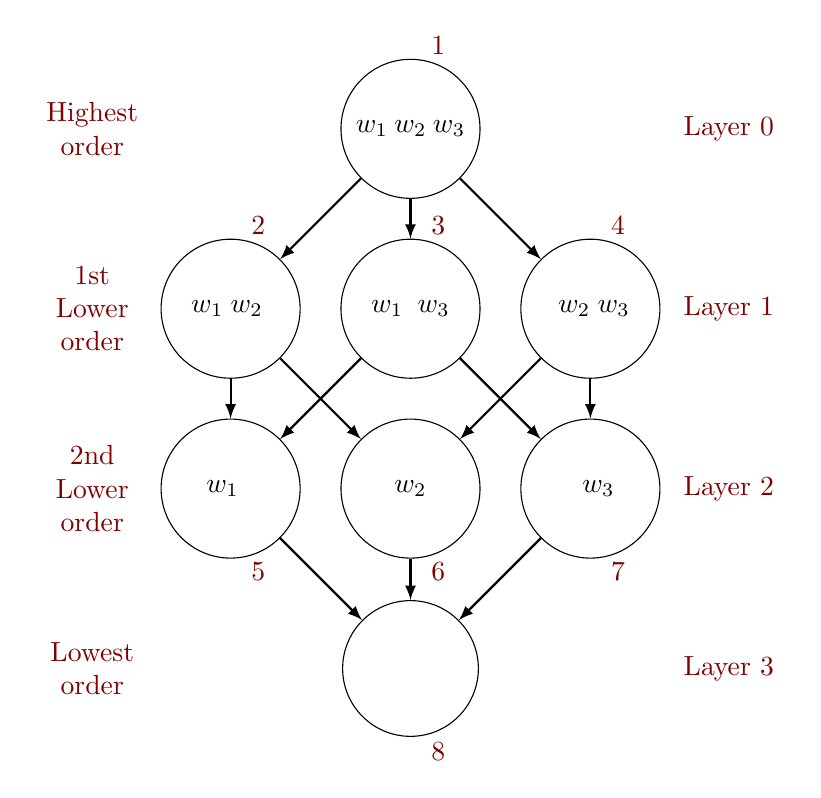
\begin{tikzpicture}
  \tikzset{
    state/.style  = {draw, circle, align = center, text centered, text width = 4.2em},
    invis/.style  = {text width = 4.2em},
    order/.style  = {align = center, text centered, text width = 4em, text = Maroon},
    number/.style = {xshift = 1em, text = Maroon},
  }

  \begin{scope}[node distance = 6.5em]
    \node [state] (000)                  {$w_1 \: w_2 \: w_3$};
    \node [invis] (000l) [left  of=000]  {};
    \node [invis] (000r) [right of=000]  {};

    \node [state] (001)  [below of=000l] {$w_1 \: w_2 \: \Skp$};
    \node [state] (010)  [below of=000]  {$w_1 \: \Skp \: w_3$};
    \node [state] (100)  [below of=000r] {$\Skp \: w_2 \: w_3$};

    \node [state] (011)  [below of=001] {$w_1 \: \Skp \: \Skp$};
    \node [state] (101)  [below of=010] {$\Skp \: w_2 \: \Skp$};
    \node [state] (110)  [below of=100] {$\Skp \: \Skp \: w_3$};

    \node [state] (111)  [below of=101] {$\Skp \: \Skp \: \Skp$};
    \node [invis] (111l) [below of=011] {};
    \node [invis] (111r) [below of=110] {};
  \end{scope}

  \begin{scope}[node distance = 5em]
    \node [order] [left of=000l]  {Highest order};
    \node [order] [left of=001]   {1st Lower order};
    \node [order] [left of=011]   {2nd Lower order};
    \node [order] [left of=111l]  {Lowest order};

    \node [order] [right of=000r] {Layer 0};
    \node [order] [right of=100]  {Layer 1};
    \node [order] [right of=110]  {Layer 2};
    \node [order] [right of=111r] {Layer 3};
  \end{scope}

  \begin{scope}[node distance = 3em]
    \node [number] [above of=000] {1};
    \node [number] [above of=001] {2};
    \node [number] [above of=010] {3};
    \node [number] [above of=100] {4};
    \node [number] [below of=011] {5};
    \node [number] [below of=101] {6};
    \node [number] [below of=110] {7};
    \node [number] [below of=111] {8};
  \end{scope}

  \path[->, >=latex, thick]
    (000) edge (001)
    (000) edge (010)
    (000) edge (100)

    (001) edge (011)
    (001) edge (101)
    (010) edge (011)
    (010) edge (110)
    (100) edge (101)
    (100) edge (110)

    (011) edge (111)
    (101) edge (111)
    (110) edge (111);
\end{tikzpicture}
\end{document}

  \caption{
    $\ProbGLM$ backoff graph of order 3 for history $h = w_1 w_2 w_3$.
  }
  \label{fig:history-glm}
\end{figure}


We also call a graph that represents the inter-dependencies of probabilities
during the calculation of $\ProbGLM{w}{h}$ the \emph{binomial diamond} of order
$n = \NGramLength{h}$, because of its diamond-like shape, and a number of
properties:

\begin{enumerate}
  \item \label{itm:num-layers} Unlike the case of Modified Kneser-Ney Smoothing
    there is no longer one clear way to define a total order of all the
    histories in the graph.
    Instead, if we partitioned the graph into layers, where layer $l$ contains
    the histories that have exactly $l$ skip words,
    the graph has $n + 1$ layers.
  \item \label{itm:num-childs} Layer $l$ contains exactly $\binom{n}{l}$ nodes.
  \item \label{itm:num-edges}  Nodes in layer $l$ have exactly $n - l$ outgoing
    and $l$ incoming edges.
  \item \label{itm:num-nodes}  There are $2^n$ nodes in the graph.
\end{enumerate}

\Cref{itm:num-layers} is due to the fact that layer $l$ includes exactly the
histories that are part of the $k$th highest order of probability.

To explain \cref{itm:num-childs}, it is helpful to imagine replacing words in
a history as laying a mask of either a skip or a non-skip on top of each word.
Then the number of nodes in each layer can be understood as permuting the
skip and non-skip masks on top of the history.
It is a well known fact that there are exactly $\binom{n}{l}$ permutations of
$l$ tokens of type A (skips) and $k$ tokens of type B (non-skips) when
$n = l + k$.

\Cref{itm:num-edges} directly follows from the fact that each non-skip word
in a history can be replaced by a skip, and that each skip is the result
of these replacements.

Last, we can explain \cref{itm:num-nodes} because every history is simply the
result of laying a mask which consists of a combination of skips or non-skips on
top of the original history.
All possible masks are therefore all permutations of two elements (skips or
non-skips) with repetition of length $n$, which there are $2^n$ arrangements of.
We can also infer this from \cref{itm:num-childs} via the binomial theorem
$(x+ y)^n = \sum_{l=0}^n \binom{n}{l} x^{n-l} y^l$, if we set ${x = y = 1}$,
we obtain $\sum_{k=0}^n \binom{n}{l} = 2^n$.

Following the model of the backoff graph will be a major aid in understanding
the weighted sum representation of the Generalized Language Model.

In order to have a notation available for all derived histories, we impose an
arbitrary total ordering on the histories.
One such ordering is given in \cref{fig:history-glm} and assigns each history
a number between $1$ and $8$.
Let $\DerivedHistory[i]$ than be the $i$th history of an arbitrary, but fixed
ordering.

% - - - - - - - - - - - - - - - - - - - - - - - - - - - - - - - - - - - - - - -
\subsection{Number of Sum Weights}

In the previous subsection, it was reasoned that, in the Generalized Language
Model, for a history of length $n$ there are exactly $2^n$ possible derivative
histories.
Following this, one might make the assumption, that to evaluate $\ProbGLM{w}{h}$
it is necessary to evaluate at most $2^n - 1$  different lower order
probabilities $\ProbGLM*{w}{\partial^* h}$ where $\partial^* h$ is any of the
$2^n - 1$ derived histories of $h$ excluding $h$ itself.
This assumption however is wrong as it can be necessary that, in the presence of
unseen histories, one history $\DerivedHistory[i]$ is both part of a highest
order probability $\ProbGLM{w}{\DerivedHistory[i]}$ and a lower order
probability $\ProbGLM*{w}{\DerivedHistory[i]}$, as will be shown in the next
paragraph.

\begin{subequations}
  Let us for example calculate the probability $\ProbGLM{w_3}{w_1 w_2}$ on
  hypothetical training data.
  That hypothetical training data shall be different from
  \cref{subsec:weightedsum-glm-example} and now $w_1 w_2$ shall be unseen,
  ergo $\Count(w_1 w_2) = 0$.
  Because of this, following \cref{eq:glm-backoff}, the average of backoff
  probabilities to be formed:
  \begin{equation}
    \ProbGLM{w_3}{w_1 w_2} = \frac{1}{2} \left( \ProbGLM{w_3}{\Skp w_2} + \ProbGLM{w_3}{w_1 \Skp}\right)
  \end{equation}
  Note that these backoff probabilities for histories $\Skp w_2$ and $w_1 \Skp$
  are still of the highest order $\ProbGLM$.
  We now further assume history $\Skp w_2$ to also not occur in training, so that
  further backoff is necessary.
  History $w_1 \Skp$ however is treated as seen:
  \begin{align}
    \label{eq:glm-example-unseen}
    \ProbGLM{w_3}{\Skp w_2} &= \ProbGLM{w_3}{\Skp \Skp} \\
    \label{eq:glm-example-seen}
    \ProbGLM{w_3}{w_1 \Skp} &= \frac{\Count(w_1 \Skp w_3) + \gamma(w_1 \Skp) \ProbGLM*{w_3}{\Skp \Skp}}
                                    {\Count(w_2 \Skp \Skp)}
  \end{align}
  We can see that $\ProbGLM{w_3}{\Skp \Skp}$ (\cref{eq:glm-example-unseen}) and
  $\ProbGLM*{w_3}{\Skp \Skp}$ (\cref{eq:glm-example-seen}) both factor into
  probability $\ProbGLM{w_3}{w_1 w_2}$.
  They would be evaluated as:
  \begin{align}
    \ProbGLM {w_3}{\Skp \Skp} &= \frac{\Count(\Skp \Skp w_3)}{\Count(\Skp \Skp \Skp)} \\
    \ProbGLM*{w_3}{\Skp \Skp} &= \frac{\ContCountIp(\WSkp \Skp \Skp w_3)}{\ContCountIp(\WSkp \Skp \Skp \WSkp)}
  \end{align}
\end{subequations}

Because of this, it is possible that one history $\DerivedHistory[\DummyIndex]$
might both occur as highest order probability
$\ProbGLM{w}{\DerivedHistory[\DummyIndex]}$ and lower order probability
$\ProbGLM*{w}{\DerivedHistory[\DummyIndex]}$.
It is non-trivial to decide exactly how many derived histories occur both as
highest and lower order probabilities, and to fit algorithms to this finding.
Consequently, we only employ an upper bound of sum weights $N$ and set all
unnecessary sum weights to zero.
An upper bound for the number of sum weights is the number of derived histories
times two, as histories can occur both in highest and lower order probabilities:
\begin{equation}
  \label{eq:weightedsum-glm-num}
  N = 2 \cdot 2^\NGramLength{h}
\end{equation}

% - - - - - - - - - - - - - - - - - - - - - - - - - - - - - - - - - - - - - - -
\subsection{Sum Terms}

Based on this we can define the sum terms for $1 \leq i \leq N$.
\begin{subequations}
  \begin{align}
    \label{eq:glmarg-high}
    \SumArg_{2 i - 1}^h(w) &=
      \begin{dcases*}
        \DiscountedCount(\DerivedHistory[i] w)        & if $\NumSkpOp{\DerivedHistory[i]} > 0$ \\
        \Count(\DerivedHistory[i] w)                  & if $\NumSkpOp{\DerivedHistory[i]} = 0$
      \end{dcases*} \\
    \label{eq:glmarg-low}
    \SumArg_{2 i}^h(w) &=
      \begin{dcases*}
        \DiscountedCount*(\WSkp \DerivedHistory[i] w) & if $\NumSkpOp{\DerivedHistory[i]} > 0$ \\
        \ContCountIp(\WSkp \DerivedHistory[i] w)      & if $\NumSkpOp{\DerivedHistory[i]} = 0$
      \end{dcases*}
  \end{align}
\end{subequations}
The terms with an odd index (\cref{eq:glmarg-high}) correspond to
$\DerivedHistory[i]$ occurring as the highest order of probability, the terms
with an even index (\cref{eq:glmarg-low}) to lower orders.
The case of $\NumSkpOp{\DerivedHistory[i]} = 0$ occurs when $\DerivedHistory[i]$
consists only of skips, it thus can no longer be backoffed, and therefore
presents the unigram case.

Finding the sum weights $\SumWeight^h_i$ is more complex.
We will first reason about how these weights have to be structured and then
give a more rigorous definition.
%We will first discuss weights for $\SumArg^h_{2 i - 1}(w)$, that is for the
%terms that compose the highest order.
The sum weights $\SumWeight^h_{2 i - 1}$, that are multiplied with
$\SumArg^h_{2 i - 1}(w)$ which compose the highest order weight, will be
discussed first.
Our solution is oriented along the backoff graph.
The weight of a history is exactly then zero, if no backoff step of
\cref{eq:glm-backoff} reaches that history.
This occurs if for that history's node all histories of immediate parent nodes
are seen.
Conversely, this means that the sum weights $\SumWeight^h_{2 i - 1}$ are proportional
to the number of paths from the root note to the current node, for which the
current node's history is seen but the histories of all others nodes in the
path are not.

What also has to be considered is that in \cref{eq:glm-backoff} we divide the
sum of all backoff probabilities by their count.
The more backoff steps that have to be performed to reach a node, the lower its
influence is.
However, in turn it also can be reached via more paths as seen in the backoff
graph of \cref{fig:history-glm}.
In total there exist two paths from the root node to any node in layer $2$.
But there exists a total of six paths from the root node to a node in layer
$3$.
We define a coefficient $\mu = \frac{(\NGramLength{h} - l_i)!}{\NGramLength{h}!}$,
where $l_i$ is the layer in the backoff graph in which the node of history
$\DerivedHistory[i]$ lies.
Sum weights $\SumWeight^h_i$ are also proportional to that coefficient $\mu$.

The final influence on $\SumWeight^h_{2 i - 1}$ stems from the fact that we
defined \cref{eq:glmarg-high} to only consist of the numerator of
\cref{eq:glm-high}.
Because of this we also have to divide the sum weight by the denominator of
that equation.

Sum weights $\SumWeight^h_{2 i}$ for terms that occur in lower orders are
calculated in an analogous way.
For the same argument as above they are also influenced by the coefficient
$\mu$ and a denominator, but this time that of \cref{eq:glm-low}.
However, for lower order weights they are also influenced by the denominators
of equations that included them.
This fact is especially visible by the nesting of fractions in
\cref{eq:probglmexpansion-inserted}.
From this equation we can conclude that a sum weight $\SumWeight^h_{2 i}$ of a
node is as sum of recursive calls from the root probability $\Prob{w}{h}$ to
the current node.
The chains of recursive calls that can reach a history $\DerivedHistory[i]$ are
exactly represented by the paths to it in the backoff graph.
Each node contributes a $\frac{\gamma}{\text{denominator}}$ weight.
Lower order sum weights thus consists of sums of multiplications, where the
factors are based on the nodes along a path to the current node.
\todo{Additional explanation of $factor \cdot sum$ property.}

Because of this complexity of terms that compose the sum weights, we will not
try to find a mathematical expression that defines these sum weights.
Instead, we will define them by specifying the algorithm that computes them:
Sum weights $\SumWeight^h_i$ are calculated by \cref{alg:weightedsum-glm} which
uses the auxiliary functions of \cref{alg:weightedsum-glm-helper}.

%\begin{algorithm}
%  \begin{algorithmic}[1]
%    \Function{calcCoefficient}{$level$, $order$}
%      \Rene[inline]{This is cached, right?}
%      \State $\mu = 1$
%      \For{$i \gets 1 \mathinner{\ldotp \ldotp} level$}
%        \State $\mu \gets \frac{\mu}{order - i + 1}$
%      \EndFor
%      \State \textbf{return} $\mu$
%    \EndFunction
%  \end{algorithmic}
%\end{algorithm}

\begin{algorithm}[t]
  \caption{Computing Generalized Language Model sum weights}
  \label{alg:weightedsum-glm}
  \begin{algorithmic}[1]
    \Require $h$
      \Comment{history for which to determinate sum weights}
    \Ensure $\SumWeight_1^h, \: \ldots, \: \SumWeight_N^h$
      \Comment{list of sum weights}

    %\State $n \gets \NGramLength{h}$
    %  \Comment{$n$-gram length of history $h$}
    \State $N \gets 2 \cdot 2^\NGramLength{h}$
      \Comment{number of sum factors}
      \label{ln:glm-numfactors}
    \For{\textbf{each} node \textbf{in} graph}
      \label{ln:glm-fornodesingraph}
      \LineComment{data lookup}
      \State node.count $\gets \Count(\DerivedHistory[\text{node.index}] \Skp)$
        \label{ln:glm-lookup-count}
      \State node.contCount $\gets \ContCountIp(\WSkp \DerivedHistory[\text{node.index}] \WSkp)$
        \label{ln:glm-lookup-contcount}
      \State node.gamma $\gets \gamma(\DerivedHistory[\text{node.index}])$
        \label{ln:glm-lookup-gamma}
      \State $\mu \gets \frac{(\NGramLength{h} - \text{node.layer})!}{\NGramLength{h}!}$
        \label{ln:glm-lookup-coeff}

      \vspace{1.0em}
      \LineComment{weight for highest order}
      \If{node.count $= 0$}
        \label{ln:glm-if-highweight-zero}
        \State $\SumWeight_{2 \cdot\, \text{node.index} - 1}^h \gets 0$
          \label{ln:glm-highweight-zero}
      \ElsIf{node $=$ root}
        \label{ln:glm-if-highweight-root}
        \State $\SumWeight_{2 \cdot\, \text{node.index} - 1}^h \gets \frac{1}{\text{node.count}}$
          \label{ln:glm-highweight-frac}
      \Else
        \label{ln:glm-if-highweight-else}
        \State $\SumWeight_{2 \cdot\, \text{node.index} - 1}^h \gets \dfrac{\mu \cdot \text{\Call{highestOrderWeight}{root, node}}}{\text{node.count}}$
          \label{ln:glm-highweight-rec}
      \EndIf

      \vspace{0.7em}
      \LineComment{weight for lower orders}
      \If{node.contCount $= 0$ \textbf{or} node $=$ root}
        \label{ln:glm-if-lowweight-zero}
        \State $\SumWeight_{2 \cdot\, \text{node.index}}^h \gets 0$
          \label{ln:glm-lowweight-zero}
      \Else
        \label{ln:glm-if-lowweight-else}
        \State $\SumWeight_{2 \cdot\, \text{node.index}}^h \gets \dfrac{\mu \cdot \text{\Call{lowerOrdersWeight}{root, node, \textbf{true}}}}{\text{node.contCount}}$
          \label{ln:glm-lowweight-rec}
      \EndIf
    \EndFor
    \algstore{glmbreak}
  \end{algorithmic}
\end{algorithm}

\begin{algorithm}[t]
  \caption{Auxiliary functions for GLM sum weight computation}
  \label{alg:weightedsum-glm-helper}
  \begin{algorithmic}[1]
    \algrestore{glmbreak}
    \Function{highestOrderWeight}{ancestor, node}
      \If{ancestor.count $\neq 0$}
        \label{ln:highhlp-count-nonzero}
        \Comment{if ancestor is seen}
        \State \textbf{return} $0$
          \Comment{this path does not contribute to highest order}
          \label{ln:highhlp-return-zero}
      \EndIf

      \vspace{0.7em}
      \If{ancestor.\Call{isParentOf}{node}}
        \label{ln:highhlp-isparent}
        \Comment{end of path?}
        \State \textbf{return} $1$
          \label{ln:highhlp-return-one}
      \EndIf

      \vspace{0.7em}
      \State sum $\gets 0$
        \label{ln:highhlp-init-sum}
      \For{\textbf{each} child \textbf{in} ancestor.\Call{childs}{$ $}}
        \label{ln:highhlp-for}
        \If{child.\Call{isAncestorOf}{node}}
          \label{ln:highhlp-isancestor}
          \State sum $\gets$ sum $+ {}$ \Call{highestOrderWeight}{child, node}
            \label{ln:highhlp-add}
        \EndIf
      \EndFor
      \State \textbf{return} sum
        \label{ln:highhlp-return}
    \EndFunction

    % --------------------------------------------------------------------------
    \vspace{0.7em}
    \Statex\hrule

    \Function{lowerOrdersWeight}{ancestor, node, firstSeen}
      \LineComment{calculate mult}
      \If{firstSeen \textbf{and} ancestor.count $\neq 0$}
        \label{ln:lowhlp-count-nonzero}
        \State factor $\gets \frac{\text{ancestor.gamma}}{\text{ancestor.count}}$
          \label{ln:lowhlp-from-highhlp}
        \State firstSeen $\gets$ \textbf{false}
          \label{ln:lowhlp-firstseen}
      \ElsIf{ancestor.contCount $\neq 0$}
        \label{ln:lowhlp-contcount-nonzero}
        \State factor $\gets \frac{\text{ancestor.gamma}}{\text{ancestor.contCount}}$
          \label{ln:lowhlp-from-lowhlp}
      \Else
        \label{ln:lowhlp-else}
        \State factor $\gets 1$
          \label{ln:lowhlp-one}
      \EndIf

      \vspace{0.7em}
      \If{ancestor.\Call{isParentOf}{node}}
        \label{ln:lowhlp-isparent}
        \Comment{end of path?}
        \If{firstSeen}
          \label{ln:lowhlp-isseen}
          \State \textbf{return} $0$
            \label{ln:lowhlp-return-zero}
            \Comment{node occurs as highest order for this path}
        \EndIf{}
        \State \textbf{return} mult
          \label{ln:lowhlp-return-mult}
      \EndIf

      \vspace{0.7em}
      \State sum $\gets 0$
        \label{ln:lowhlp-init-sum}
      \For{\textbf{each} child \textbf{in} ancestor.\Call{childs}{$ $}}
        \label{ln:lowhlp-for}
        \If{child.\Call{isAncestorOf}{node}}
          \label{ln:lowhlp-isancestor}
          \State sum $\gets$
            \label{ln:lowhlp-add-1}\\
            \hfill sum $+$ \Call{lowerOrdersWeight}{child, node, firstSeen}
            \label{ln:lowhlp-add-2}
        \EndIf{}
      \EndFor
      \State \textbf{return} factor $\cdot$ sum
        \label{ln:lowhlp-return}
    \EndFunction
  \end{algorithmic}
\end{algorithm}

The algorithm works with the notion of a backoff graph as shown in
\cref{fig:history-glm}.
That graph is unique for every history $h$ and consist of $2^\NGramLength{h}$
nodes.
Each node is assigned a derived history.
A directed edge from node $A$ to node $B$ is drawn if $B$'s history can be
created by replacing one word in $A$'s history with a skip $\Skp$.

\emph{Parents} of a node $A$ are all nodes $B$ that have a directed edge from
$B$ to $A$.
\emph{Children} of a node $A$ are all the nodes, that $A$ is a parent of.
\emph{Ancestors} of a node $A$ are all nodes that can be reached from $A$
by repeated application of the parent relation.
A \emph{path} exists to node $A_1$ from node $A_m$, if there is a set of nodes
$\Set{A_1, \ldots, A_m}$ such that it holds for all nodes $A_i$ in that set,
that $A_{i+1}$ is a parent of $A_i$ for $1 \leq i < m$.
The \emph{root} of a graph is the node that has no parents and is an ancestor
to all other nodes.
% The path to $A_1$ from $A_m$ then consists of all the nodes of that set.

To assign sum weights $\SumWeight^h_{2 i - 1}$ and $\SumWeight^h_{2 i}$ to
every history $\DerivedHistory[i]$ of the backoff graph we iterate over all
nodes in the graph in \cref{ln:glm-fornodesingraph}.
First some required data is prefetched
(\cref{ln:glm-lookup-count,ln:glm-lookup-contcount,ln:glm-lookup-gamma,ln:glm-lookup-coeff}),
then the highest order weight is computed
(\cref{ln:glm-if-highweight-zero,ln:glm-highweight-zero,ln:glm-if-highweight-root,ln:glm-highweight-frac,ln:glm-if-highweight-else,ln:glm-highweight-rec}),
and last that for lower orders
(\cref{ln:glm-if-lowweight-zero,ln:glm-lowweight-zero,ln:glm-if-lowweight-zero,ln:glm-if-lowweight-else,ln:glm-lowweight-rec}).

\emph{node.index} is simply the position of the total ordering of the backoff
graph the node got assigned.
The actual ordering does not matter, it however has to be consistent such that
$\DerivedHistory[\text{node.index}]$ is the history that belongs to that node.
Accessing a count value like $\Count(\DerivedHistory[\text{node.index}] \Skp)$
in \cref{ln:glm-lookup-count} is a potentially expensive operation, as a
separate data structure has to be queried.
\emph{node.count}, \emph{node.contCount}, and \emph{node.gamma} shall simply be
floating point variables that are stored local to each node and are thus quickly
accessible.
A possible implementation that supports this is showcased in
\cref{subsec:weightedsum-glm-implementation}.
\Cref{ln:glm-lookup-coeff} is listed under data lookup because the computation
of $\mu$ can simply be replaced by a lookup to a precomputed table with a
two-dimensional key. \emph{node.layer} is the layer of the node in the
backoff graph.

The properties \emph{node.count}, \emph{node.contCount}, and
\emph{node.gamma} are not only needed for calculations of the current node, but
also for the ones of all its descendants (for example
\cref{ln:highhlp-count-nonzero}).
Because of this an implementation has to ensure that the for-each loop in
\cref{ln:glm-fornodesingraph} only iterates over a node in layer $l$ if all
nodes of $l-1$ have been previously iterated.

Next the highest order weight $\SumWeight^h_{2 i - 1}$ is calculated.
That weight is zero if the node's history is unseen
(\cref{ln:glm-if-highweight-zero,ln:glm-highweight-zero}), as of
\cref{eq:glm-backoff}.
If the current node is the root node, we can specify the weight directly
(\cref{ln:glm-if-highweight-root,ln:glm-highweight-frac}), as of
\cref{eq:glm-high}.
Else we will have to apply the reasoning we outlined above and define the sum
weight as the fraction of coefficient $\mu$, number of paths, and denominator
(\cref{ln:glm-if-highweight-else,ln:glm-highweight-rec}).
\Call{highestOrderWeight}{\emph{ancestor}, \emph{node}} is a auxiliary function
that just counts the number of paths that only spans unseen nodes from
an \emph{ancestor} node to the current \emph{node} in a recursive manner.

Last, the weight $\SumWeight^h_{2 i}$ for lower orders is calculated.
Again if the term that would occur in the denominator \emph{node.contCount} is
zero, that term is assigned a weight of zero.
This also happens for the root note, as it can never occur in a lower order term
(\cref{ln:glm-if-lowweight-zero,ln:glm-lowweight-zero}).
Else a similar term to the highest order weight is computed, however with a
different auxiliary function
(\cref{ln:glm-if-lowweight-else,ln:glm-lowweight-rec}).

That auxiliary function \Call{lowerOrdersWeight}{\emph{ancestor}, \emph{node},
\emph{firstSeen}} forms the core of the algorithm.
We have reasoned above that the weight for lower orders is proportional to
a sum of multiplications, where each multiplication is built out of one path
from the root to the current node and each node contributes a
$\frac{\gamma}{\text{denominator}}$ factor.
This however depends on the node: if a node is the first seen one on the path
it contributes a
$\gamma(\DerivedHistory[\DummyIndex]) \div \Count(\DerivedHistory[\DummyIndex] \Skp)$
factor (\cref{ln:lowhlp-count-nonzero,ln:lowhlp-from-highhlp}) as of
\cref{eq:glm-high}. Following nodes on the path contribute a
$\gamma(\DerivedHistory[\DummyIndex]) \div \ContCount(\WSkp \DerivedHistory[\DummyIndex] \WSkp)$
factor (\cref{ln:lowhlp-contcount-nonzero,ln:lowhlp-from-lowhlp}) as of
\cref{eq:glm-low}.
Nodes that are unseen contribute the neutral element of multiplication, i.e.\
they don't change the weight (\cref{ln:lowhlp-else,ln:lowhlp-one}) as of
\cref{eq:glm-backoff}.

Also, we don't just compute sums of multiplications but instead apply
the distributive property were possible to reduce computational cost.
Each recursive step of the auxiliary function thus returns only a \emph{factor}
times \emph{sum} product, where the sum consists of incarnations of further
recursion depth
(\cref{ln:lowhlp-init-sum,ln:lowhlp-for,ln:lowhlp-isancestor,ln:lowhlp-add-1,ln:lowhlp-add-2,ln:lowhlp-return}).

% - - - - - - - - - - - - - - - - - - - - - - - - - - - - - - - - - - - - - - -
\subsection{Implementation}
\label{subsec:weightedsum-glm-implementation}

% \newlength{\oldtextfloatsep}
% \setlength{\oldtextfloatsep}{\textfloatsep}
% \setlength{\textfloatsep}{0em}

\begin{lstlisting}[
  label = {lst:backoff-graph-c},
  float,
  caption = {C data structures to implement the backoff graph},
  language = C,
]
  struct node {
    int count;
    int contCount;
    double gamma;
  };

  struct graph {
    char* history[n];
    struct node nodes[n * n]
  };
\end{lstlisting}

\begin{lstlisting}[
  label = {lst:next-in-order-index},
  float,
  caption = {C code to compute the next iteration index},
  language = C,
]
  if (index == 0)
      index = 1:
      return;

  int x = numberOfSetBits(index);

  // compute lexicographically next bit permutation
  // with x bits set
  int t = (index | (index - 1)) + 1;
  index = t | ((((t & -t) / (index & -index)) >> 1) - 1);

  // highest number with x bits set
  int m = ((1 << x) - 1) << (n - x);
  if (index > m)
      // next is smallest number with (x+1) bits
      index = (1 << (x + 1)) - 1;
  if (index > (1 << n) - 1)
      // restart, if next number would be more than n bits
      index = 0;
\end{lstlisting}

This subsection will explain our approach of implementing the backoff graph that
both consumes as little space as possible while being fast to traverse.
Our representation fits into a small contiguous amount of memory on the stack,
which will prevent cache misses, and thus result in access time improvements.

We reasoned in \cref{subsec:backoff-graph} that a backoff graph, for a history
$h$ with length $\NGramLength{h}$, has $2^\NGramLength{h}$ nodes.
Our core idea is now to store the graph into an array of $2^\NGramLength{h}$
\texttt{struct}s.

We will interpret each node's history as a binary number, where each set word
in the history becomes a zero and each skip becomes a one.
That is the node of history $w_1 \Skp w_3 w_4 \Skp$ for a graph of order $5$
is stored at the index $\texttt{01001}_2 = 9$.
That number is used as the index for each node in the array.
This representation makes it very fast to compute the layer, all parents, or
all children of a node.
These tasks can be specified entirely as bit operations, which should be
available as direct machine instructions for most architectures.
No materialized lists of all parents or all children are necessary.

The C code of \Cref{lst:backoff-graph-c} exhaustively lists necessary data
structures to implement \cref{alg:weightedsum-glm,alg:weightedsum-glm-helper}.
\texttt{n} has to be a predefined constant that specifies the (maximal) length
of histories.
The \texttt{struct} \texttt{node} consists of exactly the data members that are
used for data lookup storage in the algorithm.
\texttt{history} stores the $n$-gram $h$, and \texttt{nodes} bundles all nodes
of a graph in one instance.

We will now explain how all necessary data can be retrieved from that
representation:
\begin{itemize}
  \setlength{\itemsep}{0.4ex}
  \item The history $\DerivedHistory[i]$ of a node at index $i$ is simple
    the original \texttt{history}, where a skip $\Skp$ is placed at each
    position, where the node's index has a set bit.
  \item A node is the top root node if its index has no set bits, and in turn a
    node is the bottom leaf node if all bits in the index are set.
  \item The layer of a node is the number of set bits in its index.
  \item As explained in \cref{subsec:backoff-graph}, a node at layer $l$ has
    exactly $l$ parents and $\NGramLength{h} - l$ children.
  \item The index of the $i$th parent (child) of a node is found by unsetting
    (setting) the $i$th set (unset) bit.
  \item A node \texttt{A} is an ancestor of another node \texttt{B}
    if the bitwise and-operation on their indices returns \texttt{A}'s index
    respectively it is an descendant if the same holds for the bitwise or-
    operation:
    \begin{align*}
      \text{\texttt{A} ancestor of \texttt{B}} \: &\Leftrightarrow \: \texttt{A.index \& B.index == A.index} \\
      \text{\texttt{A} descendant of \texttt{B}} \: &\Leftrightarrow \: \texttt{A.index | B.index == B.index}
    \end{align*}
    with \texttt{\&} the bitwise-and, and \texttt{|} the bitwise-or.
\end{itemize}

The only non-trivial problem that follows from this representation is finding
the proper ordering of indices in which they should be accessed during an
in-order loop over the graph.
An in-order loop over the backoff graph iterates all nodes, such that a node
of layer $l$ is only accessed once all nodes of layer $l-1$ have been processed.

\Cref{lst:next-in-order-index} gives an algorithm in C code that generates the
next in-order index\footnote{The code to compute the lexicographically next bit
permutation is courtesy of
\mbox{\url{http://graphics.stanford.edu/~seander/bithacks.html\#NextBitPermutation}}
(accessed July 14, 2015).
It requires an architecture that stores negative integers in two's complement
format.}.
As input it requires the previous \texttt{index} and the backoff graph's order
$\texttt{n} = \NGramLength{h}$.
To ensure the fastest possible execution time the algorithm aims to be a minimal
composition of bit-level operations.

% \setlength{\textfloatsep}{\oldtextfloatsep}

% ------------------------------------------------------------------------------
\section{Monotonicity}
\label{sec:monotony}

We now want to prove that the probability definitions for Modified Kneser-Ney
Smoothing (\cref{sec:weightedsum-mkn}) and the Generalized Language Model
(\cref{sec:weightedsum-glm}) are monotonic functions on the $\SumArg^h_i(w)$.
This means that higher $\SumArg^h_i(w)$ values correspond to higher
probabilities.
We can formalize that property as:
\begin{equation}
  \big(\forall i \in \Set{1, \ldots, N}: \: \SumArg^h_i(w) \geq \SumArg^h_i(w^\prime)\big)
    \implies \Prob{w}{h} \geq \Prob{w^\prime}{h}
\end{equation}
This is an important property as it allows the application of top-$k$ joining
techniques in \cref{ch:topkjoin}.

Because we have defined these probabilities as sums of weights $\SumWeight^h_i$
multiplied with terms $\SumArg^h_i(w)$ (\cref{eq:weightedsum}), and since
addition and multiplication are trivially monotonic, it suffice to show that the
$\SumWeight^h_i$ are always non-negative to prove that our probability
definitions are monotonic.

To show that $\SumWeight^h_i$ are non-negative we take at look at their
definitions (\cref{eq:mkn-sumweight},
\cref{alg:weightedsum-glm,alg:weightedsum-glm-helper}),
and observe that they are defined as a combination (multiplication and
division) of occurrence counts $\Count(\DummyArg)$ and
$\ContCount_{1+}(\DummyArg)$, numbers of paths, and interpolation weights
$\gamma(\DummyArg)$.
Since by their nature occurrence counts and numbers of paths are natural
numbers, we only need to show that the interpolation weights
$\gamma(\DummyArg)$ are also non-negative.
These interpolation weights are defined as sums of discount values
$D_\DummyIndex$ multiplied with continuation counts
$\ContCount_\DummyIndex(\DummyArg)$ (\cref{eq:review-gamma}).
Since continuation counts again are defined as natural numbers, it remains to
prove that the discount values are non-negative.

A non-formal argument is the fact that the name and usage of discounting terms
would be nonsensical if negative values would be permitted.
Additionally we can derive this fact from the definition of the discounting
values $D_1, D_2, D_{3+}$ (\cref{eq:discounts}).
It is easy to see that these discounting values increase as the number of
n-grams $n_\DummyIndex$ in the corpus increases.
The factors $Y \frac{n_2}{n_1}$, $Y \frac{n_3}{n_2}$, $Y \frac{n_4}{n_3}$ reach
the limit of $\frac{1}{2}$ for an infinitely large corpus, and thus infinitely
large number of n-grams $n_\DummyIndex$.
As a result of the fact that these factors are limited, none of the discount
values can be negative.
Thereby we can see that our probability definitions are indeed monotonic.

\chapter{Fast Prefix Queries using Top-\emph{k} Joins}
\label{ch:topkjoin}

As motivated in the introduction, we want to solve prefix queries based
on statistical language models.
Our objective is to reduce the execution time of a high number of next word
prediction queries for arbitrary histories and prefixes.
\Cref{eq:prefixquery} shows that next word prediction queries $\NWP[p][k](h)$
are an argmax of probabilities.
To optimize query time we follow a two-pronged approach:
First we identify calculations shared by multiple probabilities and perform
them only once up front.
Secondly we try to avoid iterating the whole argument space of the argmax.
Instead, our goal is to always compute the probability for the next most
promising argument, and to terminate as soon as we are sure to have found the
$k$ words that maximize the probability.

As specified in \cref{ch:review}, each language model probability  is calculated
from occurrence counts of sequences in a corpus.
In order to avoid having to analyze the corpus on each query for its relevant
sequences, the number of occurrences for all contained sequences in a corpus is
counted up front in a learning phase.
We store these counts in a data structure that is optimized for necessary
retrieval.
We will explain this data structure and define what necessary retrieval means
in \cref{sec:completiontrie}.
Subsequently, we may persist that data, so that for each requested corpus the
necessary analysis must be performed only once.

To find the answer for a query $\NWP[p][k]{h}$, probabilities $\Prob{w}{h}$ have
to be calculated for a fixed history $h$ but many different $w$.
We have shown in \cref{ch:weightedsum} that we can represent each probability
as a weighted sum that resembles \cref{eq:weightedsum}.
The weights $\SumWeight^h_i$ of that sum are composed of exactly these counts
that are independent of the argument $w$.
This enables us to calculate the $\SumWeight_i^h$ once beforehand and reuse them
for every probability calculation of a query.
The remaining factors $\SumArg^h_i(w)$ depend on $w$.
This means we can find a function $s$ that expresses our
probabilities\footnote{The definition for $s$ is just \cref{eq:weightedsum}.
This new representation is only introduced to make it clear that given the
$\SumWeight^h_i$, the probability can be calculated from the $\SumArg^h_i(w)$.}:
\todo{It is not visible from the notation that $s$ depends on the
  $\SumWeight^h_i$.}
\begin{equation}
  \label{eq:scoringfunc}
  \Prob{w}{h} = s\left(\SumArg^h_1(w), \, \ldots, \, \SumArg^h_N(w)\right)
\end{equation}

% ------------------------------------------------------------------------------
\section{Top-\emph{k} Joining Techniques}
\label{sec:topkjoin}

The problem we are trying to solve, namely finding the $k$ words $w$ that
maximize our probability $\Prob{w}{h}$, is actually well researched under the
topic of \emph{top-$k$ joining techniques}.
The result of a join operation is the set of all combinations of tuples from
multiple data sources, where each tuple combination satisfies the \emph{join
condition}.
Top-$k$ joins are then these joins that only return the $k$ highest scoring
according to some \emph{scoring function}.

We can easily see that our prefix queries fit the scheme of top-$k$ join
queries.
To calculate the probability of any word $w$, we have to look up all
$\SumArg^h_i(w)$ that belong to that word.
Finding all combinations
$\left(\SumArg^h_1(w), \, ..., \, \SumArg^h_N(w)\right)$
for each word $w$ is actually a join operation with the join condition that
the $w$ is constant over the $\SumArg^h_i(w)$ of a single combination.
As defined, for a query $\NWP[p][k]{w}$ we only want to return the $k$ best
predictions.
The $k$ best predictions are the ones that yield the $k$ highest values
according to a scoring function, which in our case is the probability.
Each join combination gives the arguments for the scoring function, as shown
in \cref{eq:scoringfunc}.

Almost all top-$k$ joining techniques that try to be more efficient than
iterating all join combinations, require \emph{monotonic} scoring functions.
Monotonicity in our context means that higher $\SumArg^h_i(w)$ values correspond
to higher probabilities.
We have shown in \cref{sec:monotony} that our probability definitions are
monotonic on the $\SumArg^h_i(w)$.
This fact can be utilized to find the top-$k$ predictions by always calculating
the probability for the next promising $w$ with the highest $\SumArg^h_i(w)$.

Finding the $w$ with the highest $\SumArg^h_i(w)$ requires sorting.
Since join combinations
$\left(\SumArg^h_1(w), \, ..., \, \SumArg^h_N(w)\right)$ are $N$-dimensional
there is no meaningful order defined on them, besides sorting by the scoring
function.
However, that requires calculating the probability for each join
combination, which is precisely what we are trying to avoid.
For this reason we instead maintain $N$ data relations, one for each
$\SumArg^h_i(w)$, and sort them independently in the learning phase.
During query time, we can then perform \emph{sorted access} on these relations,
that is for a given history $h$ we want to retrieve words $w$ paired with and
sorted by their $\SumArg^h_i(w)$.
Some top-$k$ joining techniques additionally require \emph{random access},
that is for a given history $h$ and a given word $w$ we want to find
$\SumArg^h_i(w)$.
The data structure we use for this will be explained in
\cref{sec:completiontrie}.

Among other things, top-$k$ joining techniques can be classified by the type
of join operation they support \parencite{Ilyas2008}.
The join operation for our problem is whether for two values $\SumArg^h_i(w_x)$
and $\SumArg^h_j(w_y)$ the $w_x$ and $w_y$ are equal.
This is actually the simplest and most common type of join operation and is
called an \emph{equi-join}.
They have the nice property that for each $\SumArg^h_i(w)$ there is exactly one
corresponding $\SumArg^h_j(w)$ for all $j$ that are different from $i$, which
allows easy indexing in a hash table by the key $w$.
Top-$k$ joining techniques that operate on equi-joins are also called
\emph{top-$k$ selections} \parencite{Ilyas2008}.

Two fundamental algorithms were discovered by \textcite{Fagin2001} and other
authors independently: the \emph{threshold algorithm}, which requires sorted and
random access, and the \emph{no random access algorithm}, which only requires
sorted access.
We will apply these two algorithms to the problem of next word prediction and
compare them against each other and the simple argmax approach.
\textcite{Fagin2001} prove that both these algorithms are \emph{instance
optimal} solutions to top-$k$ join queries: there is no possible algorithm
that provides a better solution over all possible database contents.

However, algorithms which outsource some computation into a precompution step,
and thus achieve a faster query response, are still possible:
there exists a plethora of such more sophisticated top-$k$ joining techniques,
of which \textcite{Ilyas2008} surveys a wide number.
For example, \emph{onion indices} \parencite{Chang2000} and
\emph{rank join indices} \parencite{Tsaparas2003} feature an extended learning
phase, in which optimized data representation are created over all arguments to
the scoring function.
These allow faster top-$k$ joins for arbitrary scoring functions over the same
arguments.
However, optimizations like these are not applicable to our prefix query problem,
as the history $h$ changes with each query $\NWP[p][k](h)$.
Because of this the whole argument space $\SumArg^h_i(w)$ changes, which in turn
means we would have to built indices with each query, obviously defeating the
purpose.
The \emph{Rank Join operator} \parencite{Ilyas2004} is another more recent
algorithm, designed for fast solution in the presence of arbitrary join
conditions.
However, in the presence of an equi-join it practically reduces to the threshold
algorithm.

% ------------------------------------------------------------------------------
\section{Corpus Data Structure: Completion Trie}
\label{sec:completiontrie}

For our needs we require a data structure that can return sorted pairs
$\left(w, \SumArg^h_i(w)\right)$ for each $i$ and a given history $h$.
Additionally as we are solving prefix queries, it has to be possible to specify
a prefix $p$ which all $w$ have to start with.

On top of that the threshold algorithm requires random access to the data
structure, that is for a given $w$ we want to find $\SumArg^h_i(w)$.
Random access might yield additional information to an algorithm and thus allow
it to terminate earlier.
Also, our definitions to calculate the sum weights $\SumWeight^h_i$ given in
\cref{ch:weightedsum} require this form of random access, so it is desirable for
our data structure to support it.
The alternative would be to maintain a separate data store that is optimized for
random access --- for example a hash map --- which would necessitate a huge
memory usage.

Another desirable characteristic of data storage is data compression.
Since the analyzation of larger corpora yields to more accurate language
models\noref, a higher degree of data compression allows to perform more
accurate word prediction on the same hardware.
Obviously a balance between data compression and access time has to be found,
since fast prefix queries are the goal of this thesis.

The data structure which satisfies all these requirements is the
\emph{completion trie} described by \textcite{HsuOttaviano2013}.
A completion trie is a compact prefix tree that allows storage of arbitrary
pairs of strings and integer-scores.
A prefix tree is an ordered tree data structure where each node stores a
character sequence.
Retrieving a full string from the trie is done by concatenating all character
sequences along a path from the root to a leaf node.
In a completion trie each node also stores the highest score of all its leaf
nodes.
This enables very fast retrieval of all string-score-pairs sorted by score,
where the string start with a requested prefix, hence the name
\emph{completion} trie.

\textcite{HsuOttaviano2013} devise a method for storing only a minimal number of
tree edges, while maintaining data locality.
Further employing a variable-byte encoding they report an average compression
ratio of their data structure of 51\% compared to raw uncompressed text files.
In the same publication \textcite{HsuOttaviano2013} present two alternative
data structures for the same task that achieve compression ratios of 29\%
respectively 30\%.
However, they report access times which are at least twice as high as the ones
of the completion trie.
Since speed is the primary concern of this thesis these alternatives
were not further considered.

For $1 \leq i \leq N$ we maintain $N$ many completion trie instances and store
pairs $\left(h \NGramConcat w, \SumArg^h_i(w)\right)$ in each trie for all possible
histories $h$ and words $w$, where $h \NGramConcat w$ is the concatenation of
$h$ and $w$.
This enables all our desired accessing schemes:
\begin{itemize}
  \item Sorted access for some history $h$ is done by querying for completions
    of $h$.
    \todo{Actually $\hat h$.}
    Results are then pairs where the string starts with the requested
    history.
    The remaining part of the string is the word $w$.
    Results are sorted on the score $\SumArg^h_i(w)$.
    \todo{Querying $i$-th trie is only said implicitly.}
  \item A prefix $p$ which $w$ has to start with is easily included.
    Querying for completions of $h \NGramConcat p$ returns the same pairs as
    above, but only the ones where $p$ is a prefix in $w$.
  \item Random access for a fixed history $h$ and fixed word $w$ is achieved by
    walking the path along the trie that is described by $h \NGramConcat w$.
    If that path ends in a leaf node, this node's score is $\SumArg^h_i(w)$.
    If that path does not exist, or the found node is not a leaf node,
    $\SumArg^h_i(w)$ is zero.
\end{itemize}

% ------------------------------------------------------------------------------
\section{Threshold Algorithm}
\label{sec:thresholdalgorithm}

The \emph{Threshold Algorithm}, applied to our problem $\NWP[p][k](w)$, roughly
works as follows \parencite{Fagin2001}:
\begin{enumerate}
  \item We perform sorted access to data sources (in our case completion tries
    are queried with prefix $h \NGramConcat p$) in any order.
    One strategy might be a round robin approach, that is each source is
    accessed once in turn.
  \item Every time a pair $(w, \SumArg^h_i(w))$ is encountered with a new word
    $w$, we look up all other $\SumArg^h_j(w)$ for $j \neq i$ with random
    access.
    With these the word probability
    $\Prob{w}{h} = s(\SumArg^h_1, \ldots, \SumArg^h_N)$ can be calculated.
    We keep track of the $k$ pairs $(w, \: \Prob{w}{h})$ with the highest
    probabilities.
  \item Let $\overline{\SumArg}_i$ denote the last count $\SumArg^h_i(w)$ that
    was encountered during sorted access to the $i$th data source.
    Then the \emph{threshold}
    $t = s(\overline{\SumArg}_1, \ldots, \overline{\SumArg}_N)$
    is an upper bound for the probability of all words that have not been
    seen yet.
  \item Once we have encountered $k$ probabilities greater than the current
    threshold $t$ the algorithm terminates and the $k$ best pairs
    $(w, \: \Prob{w}{h})$ are returned.
\end{enumerate}

\begin{algorithm}
  \caption{\emph{Threshold Algorithm} to solve $\NWP[p][k]{h}$}
  \label{alg:thresholdalgorithm}
  \begin{algorithmic}[1]
    \Require $C_1, \: \ldots, \: C_N$
      \Comment{corpus data stored in Completion Tries}
    \Require $history$, $prefix$, $limit$
    \Statex \Comment{history $h$, prefix $p$ and limit $k$ for prefix query $\NWP[p][k]{h}$}
    \Ensure $predictions$
      \Comment{list of word-probability-pairs}

    \State $\SumWeight_1, \: \ldots, \: \SumWeight_N \gets$ \Call{calcSumWeights}{history}
      \Comment{see \cref{ch:weightedsum}}
      \label{ln:ta-sumweights}
    \For{$i$ \textbf{from} $1$ \textbf{to} $N$}
      \label{ln:ta-bara-for}
      \State $\overline{\SumArg}_i \gets C_i$.\Call{peekCount}{history $\NGramConcat$ prefix}
        \Comment{threshold factors}
        \label{ln:ta-bara-peek}
    \EndFor
    \State seen $\gets$ \textbf{new} \Call{Set}{$ $}
      \Comment{set of seen words}
      \label{ln:ta-seen}
    \State queue $\gets$ \textbf{new} \Call{PriorityQueue}{$ $}
      \Comment{prediction candidates}
      \label{ln:ta-queue}

    \vspace{0.7em}
    \While{$i \gets$ \Call{nextTrie}{$ $}}
      \LineComment{perform sorted access, track seen words}
      \label{ln:ta-while}
      \State word$,$ count $\gets C_i$.\Call{next}{history $\NGramConcat$ prefix}
        \label{ln:ta-next}
      \If{seen.\Call{contains}{word}}
        \label{ln:ta-isseen-if}
        \State \textbf{continue}
          \Comment{skip words already seen in previous iterations}
          \label{ln:ta-isseen-continue}
      \EndIf
      \vspace{-1.2em} % TODO: how is the gap created we are hotfixing here?
      \State seen.\Call{add}{word}
        \label{ln:ta-seen-add}

      \vspace{0.7em}
      \LineComment{compute word probability}
      \For{$j$ \textbf{from} $1$ \textbf{to} $N$}
        \If{j == i}
          \State $\SumArg_j \gets$ count
            \label{ln:ta-a-sorted}
        \Else
          \State $\SumArg_j \gets C_j$.\Call{get}{history $+$ word}
            \Comment{random access}
            \label{ln:ta-a-random}
        \EndIf
      \EndFor
      \State probability $\gets \sum_{j = 0}^N \SumWeight_j \SumArg_j$
        \label{ln:ta-prob}

      \vspace{0.7em}
      \LineComment{keep limit-many best predictions}
      \State queue.\Call{push}{(word, probability)}
        \label{ln:ta-queue-add}
      \If{queue.\Call{size}{$ $} $>$ limit}
        \label{ln:ta-queue-full}
        \State queue.\Call{removeLowestProbabilityEntry}{$ $}
          \label{ln:ta-queue-remove}
      \EndIf

      \vspace{0.7em}
      \LineComment{compute threshold}
      \State $\overline{\SumArg}_i \gets \SumArg_i$
        \label{ln:ta-bara-update}
      \State threshold $\gets \sum_{j = 0}^N \SumWeight_j \overline{\SumArg}_j$
        \label{ln:ta-threshold}

      \vspace{0.7em}
      \LineComment{stop if better predictions are impossible}
      \If{queue.\Call{size}{$ $} $=$ limit \textbf{and}
        \label{ln:ta-done-if-1}
        \\\hspace{2.5em}threshold $<$ queue.\Call{getLowestProbability}{$ $}}
        \label{ln:ta-done-if-2}
        \State \textbf{break}
          \label{ln:ta-done-break}
      \EndIf
    \EndWhile

    \vspace{0.7em}
    \State predictions $\gets$ queue.\Call{toList}{$ $}
      \label{ln:ta-tolist}
  \end{algorithmic}
\end{algorithm}

Our implementation of the \emph{Threshold Algorithm} is given in
\cref{alg:thresholdalgorithm}.

As input we require $N$ completion tries from which we can extract
$(w, \: \SumArg^h_i(w))$ pairs in sorted or random order as described in
\cref{sec:completiontrie}.
Further, as we are finding answers to an $\NWP[p][k]{h}$ query, these parameters
$p$, $k$ and $n$ are necessary.
Both \emph{history} and \emph{prefix} are strings that may be empty;
\emph{limit} has to be an integer greater zero.
The output \emph{predictions} will be a list composed of at most
\emph{limit} $(w, \: \Prob{w}{h})$ pairs, sorted by probability in descending
order.

The calculation of probabilities depends on sum weights
$\SumWeight_1, \: \ldots, \: \SumWeight_N$.
They only depend on the fixed \emph{history} and can thus be computed once at
the start of each query (\cref{ln:ta-sumweights}).
To calculate the \emph{threshold}, the upper bound for all of remaining
probabilities, the factors
$\overline{\SumArg}_1, \: \ldots, \: \overline{\SumArg}_N$ are required.
They are the last accessed counts $\SumArg_i(w)$ of each trie.
Before performing any trie-access we initialize them to the highest count in the
trie (\cref{ln:ta-bara-for,ln:ta-bara-peek}).
\emph{Peeking} a data source is the operation that returns the next entry in it,
without advancing its iterator.

\emph{seen} is a set that keeps track of all processed words thus far
(\cref{ln:ta-seen}).
Its purpose is to avoid random access for the calculation of probabilities
that have been performed before.
It is an optimization that enables a faster execution time at the cost of
a higher space complexity.\todo{HashSet}

\emph{queue} keeps track of the word-probability-pairs with the highest
probabilities that are candidates for prediction (\cref{ln:ta-queue}).
At any point in time it contains at most $\text{\emph{limit}} + 1$ entries.
It is implemented as a priority queue, which we expect to be ordered on
the probabilities of each entry.
Thus efficient querying (\cref{ln:ta-done-if-2}) or removal
(\cref{ln:ta-queue-remove}) of the entry with the lowest probability is
possible.

After initialization is done we query words until we have found the \emph{limit}
best predictions.
The \Call{nextTrie}{$ $} function in \cref{ln:ta-while} returns the number $i$
of the trie to be queried next.
It is thus stateful and needs to keep track of previous return values.
In our implementation we perform a round-robin approach: tries are
returned in the order $1, 2, \ldots, N, 1, 2, \ldots$
Once a trie is depleted it is omitted.

For each iteration we perform sorted access and retrieve the next
word-count-pair from the current trie, that starts with the requested
\emph{history} and \emph{prefix} (\cref{ln:ta-next}).
The \Call{next}{$\DummyArg$} method of a trie returns the current pair under
the iterator and advances it in sorted order.
If the word has been encountered in a previous iteration from a different trie
we continue with the next iteration step
(\cref{ln:ta-isseen-if,ln:ta-isseen-continue}).
If the word is new, we add it to the list of seen words (\cref{ln:ta-seen-add}).

In the following, the probability $\Prob{w}{h}$ for the word is calculated
(\cref{ln:ta-prob}).
The factor $\SumArg_i$ is known from sorted access (\cref{ln:ta-a-sorted}), all
other $\SumArg_j$ with $j \neq i$ are retrieved by random access
(\cref{ln:ta-a-random}).
With the word's probability we update our record of the \emph{limit} best
predictions thus far
(\cref{ln:ta-queue-add,ln:ta-queue-full,ln:ta-queue-remove}).
The sorting of the priority queue happens implicit with the
\Call{push}{$\DummyArg$} operation.

Afterwards the last accessed sorted count of the current trie is updated
(\cref{ln:ta-bara-update}) and with it the \emph{threshold} calculated
(\cref{ln:ta-threshold}).
If we already found \emph{limit} predictions and the probability of all these
predictions is higher than our upper bound of all remaining ones, the algorithm
terminates (\cref{ln:ta-done-if-1,ln:ta-done-if-2,ln:ta-done-break}).
The resulting \emph{predictions} are formed by the conversion of the
\emph{queue} to a list (\cref{ln:ta-tolist}), where the sorting of the
\emph{queue} is respected.

% ------------------------------------------------------------------------------
\section{No Random Access Algorithm}
\label{sec:norandomaccessalgorithm}

The \emph{No Random Access Algorithm}, applied to our problem $\NWP[p][k](w)$,
roughly works as follows \parencite{Fagin2001}:
\begin{enumerate}
  \item We perform sorted access to data sources (in our case completion tries
    are queried with prefix $h \NGramConcat p$) in any order.
    One strategy might be a round robin approach, that is each source is
    accessed once in turn.
  \item We maintain a mapping that initially maps all words to \emph{unknown}
    counts $\SumArg^h_i(w)$.
    For every word-count pair queried, we set that count in the mapping to its
    now know value.
  \item Using this mapping we calculate upper and lower bounds for all seen
    words.
    Let $\overline{\SumArg}_i$ denote the last count $\SumArg^h_i(w)$ that
    was encountered during sorted access to the $i$th data source.
    The upper bound for a word probability is calculated by replacing unknown
    counts with their highest possible value $\overline{\SumArg}_i$.
    Lower bounds are calculated by replacing unknown counts with zeros.
  \item Once $k$ words have been found, whose lower bound of probability is
    higher than all other upper bounds, the algorithm terminates and returns
    these $k$ best predictions.
\end{enumerate}

\begin{algorithm}
  \caption{\emph{No Random Access Algorithm} to solve $\NWP[p][k]{h}$}
  \label{alg:norandomaccessalgorithm}
  \begin{algorithmic}[1]
    \Require $C_1, \: \ldots, \: C_N$
      \Comment{corpus data stored in Completion Tries}
    \Require $history$, $prefix$, $limit$
    \Statex \Comment{history $h$, prefix $p$ and limit $k$ for prefix query $\NWP[p][k]{h}$}
    \Ensure $predictions$
      \Comment{list of words}

    \State $\SumWeight_1, \: \ldots, \: \SumWeight_N \gets$ \Call{calcSumWeights}{history}
      \Comment{see \cref{ch:weightedsum}}
      \label{ln:nra-sumweights}
    \For{$i$ \textbf{from} $1$ \textbf{to} $N$}
      \label{ln:nra-bara-for}
      \State $\overline{\SumArg}_i \gets C_i$.\Call{peekCount}{history $\NGramConcat$ prefix}
        \label{ln:nra-bara-peek}
    \EndFor
    \State wordCounts $\gets$ \textbf{new} \Call{Map}{$ $}
      \Comment{map from words to their counts}
      \label{ln:nra-wordcounts}
    \State queue $\gets$ \textbf{new} \Call{PriorityQueue}{$ $}
      \Comment{all predictions}
      \label{ln:nra-queue}
    \State predictions $\gets$ \textbf{new} \Call{List}{$ $}
      \label{ln:nra-predictions}

    \vspace{0.7em}
    \While{$i \gets$ \Call{nextTrie}{$ $}}
      \label{ln:nra-while}
      \LineComment{perform sorted access, track known counts per word}
      \State word$,$ count $\gets C_i$.\Call{next}{history $\NGramConcat$ prefix}
        \label{ln:nra-next}
      \If{\textbf{not} wordCounts.\Call{contains}{word}}
        \label{ln:nra-contains}
        \State $\SumArg_1, \: \ldots, \: \SumArg_N \gets $ \textbf{unknown}$, \: \ldots, \:$\textbf{unknown}
          \label{ln:nra-set-unkown}
      \Else
        \State $\SumArg_1, \: \ldots, \: \SumArg_N \gets $ wordCounts.\Call{get}{word}
          \label{ln:nra-get-wordcounts}
        \State queue.\Call{remove}{word}
          \label{ln:nra-queue-remove}
      \EndIf
      \State $\SumArg_i \gets$ count
        \label{ln:nra-a-set}
      \State wordCounts.\Call{set}{word, $(\SumArg_1, \: \ldots, \: \SumArg_N)$}
        \label{ln:nra-update-mapping}

      \vspace{0.7em}
      \LineComment{compute word probability upper- and lower-bound}
      \State $\overline{\SumArg}_i \gets \SumArg_i$
        \label{ln:nra-bara-update}
      \State upperBound $\gets 0$
        \label{ln:nra-upperbound-init}
      \State lowerBound $\gets 0$
        \label{ln:nra-lowerbound-init}
      \For{$j$ \textbf{from} $1$ \textbf{to} $N$}
        \If{$\SumArg_j =$ \textbf{unknown}}
          \State upperBround $\gets$ upperBound $+ \SumWeight_j \overline{\SumArg}_j$
            \label{ln:nra-upperbound-unknown}
        \Else
          \State upperBound $\gets$ upperBound $+ \SumWeight_j \SumArg_j$
            \label{ln:nra-upperbound-known}
          \State lowerBound $\gets$ lowerBound $+ \SumWeight_j \SumArg_j$
            \label{ln:nra-lowerbound-known}
        \EndIf
      \EndFor

      \vspace{0.7em}
      \LineComment{predict words with lower bound $\geq$ all other upper bounds}
      \State queue.\Call{push}{(word, upperBound, lowerBound)}
        \label{ln:nra-queue-push}
      \While{\textbf{true}}
        \label{ln:nra-while-true}
        \State word, upperBound, lowerBound $\gets$ queue.\Call{pop}{$ $}
          \label{ln:nra-queue-pop}
        \If{lowerBound $\geq$ queue.\Call{getLargestUpperBound}{$ $}}
          \label{ln:nra-lowerbound-greater}
          \State predictions.\Call{add}{word}
            \label{ln:nra-certain-predict}
        \Else
          \State queue.\Call{push}{(word, upperBound, lowerBound)}
            \label{ln:nra-queue-readd}
          \State \textbf{break}
            \label{ln:nra-predict-break}
        \EndIf
        \If{predictions.\Call{size}{$ $} $=$ limit}
          \label{ln:nra-isdone}
          \State \textbf{exit}
            \label{ln:nra-exit}
        \EndIf
      \EndWhile
    \EndWhile

    \vspace{0.7em}
    \For{$i$ \textbf{from} predictions.\Call{size}{$ $} \textbf{to} limit}
      \label{ln:nra-for-limit}
      \State word, upperBound, lowerBound $\gets$ queue.\Call{pop}{$ $}
        \label{ln:nra-pop-2}
      \If{upperBound $= 0$}
        \label{ln:nra-upperbound-zero-if}
        \State \textbf{break}
          \label{ln:nra-upperbound-zero-break}
      \EndIf
      \State predictions.\Call{add}{word}
        \label{ln:nra-limit-predict}
    \EndFor
  \end{algorithmic}
\end{algorithm}

\Cref{alg:norandomaccessalgorithm} shows our implementation of the
\emph{No Random Access Algorithm}.

The input requirements are the same as for the \emph{Threshold Algorithm}
described in \cref{sec:thresholdalgorithm}.
The output is similar, however we only return a list of predicted words without
their probabilities, as the algorithm doesn't compute the exact probabilities.
Also the initialization of sum weights
$\SumWeight_1, \: \ldots, \: \SumWeight_N$ and last seen counts
$\overline{\SumArg}_1, \: \ldots, \: \overline{\SumArg}_N$ is the same as
before (\cref{ln:nra-sumweights,ln:nra-bara-for,ln:nra-bara-peek}).

\emph{wordCounts} is the mapping from words $w$ to $N$-tuples that contain the
counts $\SumArg^h_i(w)$ (\cref{ln:nra-wordcounts}).
Unset values are interpreted as having \emph{unknown} counts.

\emph{queue} is a priority queue that stores $($word$,$ upper
bound$,$ lower bound$)$ tuples (\cref{ln:nra-queue}).
As opposed to the \emph{Threshold Algorithm} the queue needs to keep track of
bounds for all encountered words, not just \emph{limit} many.
Entries in the queue are sorted by lower bounds and for objects with equal
lower bounds sorted by their upper bounds.

\emph{predictions} is the list of all possible word predictions
(\cref{ln:nra-predictions}).
Words in the list are sorted by probability descending without actually
calculating the probability.
It contains at most \emph{limit} items.

The selection of the next trie with \Call{nextTrie}{$ $} (\cref{ln:nra-while})
and the following sorted access to that trie (\cref{ln:nra-next}) are equal
to the ones of the \emph{Threshold Algorithm}.
Each new word-count-pair is stored in \emph{wordCounts}.
If the word has not been seen before (\cref{ln:nra-contains}) we initialize all
counts $\SumArg_1, \: \ldots, \: \SumArg_N$ as \emph{unknown} values.
Otherwise we load previously stored counts from the mapping
(\cref{ln:nra-get-wordcounts}).
Additionally as we know the word to receive updated bounds its entry is removed
from the \emph{queue} (\cref{ln:nra-queue-remove}).
Afterwards we update the one $\SumArg_i$ we have retrieved the value for
(\cref{ln:nra-a-set}) and write the resulting count-tuple back into the map
(\cref{ln:nra-update-mapping}).

With the updated counts we can compute a better upper and lower bound for the
word probability.
First we update the last accessed count of the current trie
(\cref{ln:nra-bara-update}).
Bounds are then calculated as the weighted sums of $\SumArg_j$
(\cref{ln:nra-upperbound-known,ln:nra-lowerbound-known}).
In case the the value of any $\SumArg_j$ is \emph{unknown}, it is  substituted
with the highest possible value $\overline{\SumArg}_j$ for the calculation of
the upper bound (\cref{ln:nra-upperbound-unknown}) or in the case of the lower
bound it is not factored in at all.

The newly calculated bounds of the word are then added to the \emph{queue}
(\cref{ln:nra-queue-push}).
Afterwards all words that have a higher lower bound than the largest
upper bound of all other words in the queue are added as final
\emph{predictions}.
First the next word with the highest lower bound is retrieved from the queue
with the \Call{pop}{$ $} operation (\cref{ln:nra-queue-pop}).
If that word's lower bound is greater or equal to the largest remaining upper
bound in the queue (\cref{ln:nra-lowerbound-greater}) we can add it to the list
of \emph{predictions} (\cref{ln:nra-certain-predict}) and repeat the process.
Otherwise we add the word back into the queue and continue with new sorted
retrieval.
The algorithm terminates once \emph{limit} predictions have been found
(\cref{ln:nra-isdone,ln:nra-exit}).
This procedure ensures that predictions are added in order of decreasing
probabilities.

Attention must be paid to the upper bounds of all objects in the \emph{queue}.
Technically whenever an $\overline{\SumArg}_i$ value is updated, the upper bound
of each item in the queue, for with $\SumArg_i$ is unknown, will change.
So in practice one would have to recalculate all upper bounds and resort the list
every time an $\overline{\SumArg}$ value is updated.
This is not made explicit in the presented algorithm.
However, one can take advantage of the fact that our probabilities are
monotonic, and the sorting of items thus remains constant for changing
$\SumArg_i$.
This means one only needs to recalculate the upper bound in places where the
actual value is needed.

A case than can occur for small corpora, is that all tries may be depleted
before \emph{limit} predictions have been established.
Because of this we fill the \emph{predictions} with words from the \emph{queue}
in order until \emph{limit} many have been reached
(\cref{ln:nra-for-limit,ln:nra-pop-2,ln:nra-upperbound-zero-if,ln:nra-upperbound-zero-break,ln:nra-limit-predict}).
However, if remaining words have a probability upper bound of zero
(\cref{ln:nra-upperbound-zero-if}) we prefer to have less than \emph{limit}
predictions, as the remaining ones are guaranteed not to match.

% ------------------------------------------------------------------------------
\clearpage
\section{Implementation}

Previously we have spoken about querying a completion trie with a history
$h$ and retrieving a pair $(w, \SumArg^h_i(w))$.
However, this is only a simplified view on the underlying process.
In practice it is infeasible to store $\SumArg^h_i(w)$ for every possible
history $h$, or even only for seen histories.
Instead we rely on the derived histories $\DerivedHistory[\DummyIndex]$
(\cref{fig:history-mkn,fig:history-glm}), described in \cref{ch:weightedsum},
which overlap for multiple query histories $h$.
So to obtain an $\SumArg^h_i(w)$, the $i$th completion trie has to be queried
with $\DerivedHistory[i]$.
Deriving the $\DerivedHistory[\DummyIndex]$ from $h$ is possible via simple
computation rules.

An operation like $C_i$.\Call{next}{$\DummyArg$} obviously incurs a notion
of state to enable access to the \emph{next} object.
This state is unique to each instance of the algorithm and each completion trie.
In our implementation we use iterators to abstract this away.
This is not made explicit in the shown algorithms.

In the algorithms we select the next trie to query by the method
\Call{nextTrie}{$ $}.
This call abstracts the problem of finding the optimal next trie.
As we have said, all access strategies are possible, as long as empty tries ---
tries whose iterator has passed the last entry --- are not selected anymore.
A simple strategy is round robin access, that is accessing each trie after
another and then starting over.
\textcite{Guentzer2000,Guentzer2001} research optimal access strategies for
both presented algorithms.
They introduce a notion of the partial derivative of a data source to find the
most efficient next trie.

Another thing related to empty tries is that the last seen count
$\bar{\SumArg}_i$ needs to be set to zero once the $i$th trie is depleted.
Else a terminating state might never be reached.

\begin{draft}
Can't actually store $\SumArg(\DummyArg)$ but only counts $\Count(\DummyArg)$.
Discounts fuck everything up and sometimes require random access even when only
doing sorted.
\end{draft}

% ------------------------------------------------------------------------------
\section{Discussion}

We will now discuss advantages and disadvantages of both algorithms.
On average the Threshold Algorithm will be able to terminate much faster,
because it has access to additional information obtained via random accesses.
The No Random Access Algorithm only performs sorted access and has to perform
additional book keeping in order to compute its results.
This results in a longer runtime and higher memory requirements.

Both algorithms need to keep track of all word they have encountered through
sorted access.
On top of that the top-$k$ joining algorithm only needs to keep track of at most
$k$ word-probabilities pairs.
The number of predictions $k$ is usually small --- on current smartphones one
to five --- so this can be neglected.
The No Random Access Algorithm on the other hand needs to keep track of all
encountered occurrence counts plus upper and lower probability bounds, so has
considerably steeper memory requirements.

The runtime of both algorithms is largely dependent on the costs of sorted and
random access.
For our application and data structure we perform an in-depth empirical
comparison in \cref{subsec:evaluation-topkjoin-time}.
In our setup the Threshold Algorithms performs its calculations much more
quickly for the vast share of queries.
\textcite{Fagin2001} present the \emph{Combined Algorithm}, a generalized
version of both, that performs an optimal ratio of sorted and random accesses,
if the runtime costs of both forms of access are known.
Finding the correct access costs for top-$k$ joining next word prediction and
fitting the Combined Algorithm to these would be interesting future work.

For our application of word prediction the Threshold Algorithm is superior in
all metrics and should be preferred in practice.
The strength of the No Random Access Algorithm is that it can still be used in
systems where random access is impossible to implement.
These types of systems are imaginable in distributed systems were each node only
stores part of a language model.

% ------------------------------------------------------------------------------
\iffalse
\begin{draft}
\section{Alternatives}

Why beam search is impossible.

Beam search is a path finding algorithm that always expands the most promising
states, and terminates when a solution was found.

This however is not directly applicable to our problem, as finding a solution
is typically very easy (get top node from sorted pattern counts and take it as
solution).

How to interpret: expanding the most promising state?
\begin{enumerate}
  \item Peek sorted counts, list with highest count is most promising.
  \item Now how to determine if we want to do random access to missing pattern
    counts or rather fetch next sorted count.
  \item Could do beam width many sorted accesses, and complete missing patterns
    with random acccess and call it a day.
\end{enumerate}

For random access the cost of an edge is only known, once the edge is walked.
For sorted access we can peek.
\end{draft}
\fi

\chapter{Evaluation}

\begin{draft}
GLMTK by me was used for evaluation.

Experiment with runtime of $\ProbGLM{w_n}{w_1^{n-1}}$ from $n=1$ to some upper
bound to showcase complexity improvement of weighted sum to na{\"\i}ve,
recursive approach.

Experiment with top-k join algorithm vs stupid weighted sum argmax, to showcase
runtime improvement of top-k join.

Experiment to showcase (dis-)advantages of GLM to MKN.

Maybe Speedup-factor over time.

Experiments that combine metrices.

Experiments over time and space complexity.
\end{draft}

% ------------------------------------------------------------------------------
\section{Experimental setup}

% ------------------------------------------------------------------------------
\section{Estimator time}

\begin{figure}
  \centering
  \documentclass{standalone}
\usepackage[dvipsnames,svgnames,x11names]{xcolor}
\usepackage{tikz}
\usepackage{pgfplots}
\pgfplotsset{compat = 1.12}
\usepackage{../thesismath}
\begin{document}
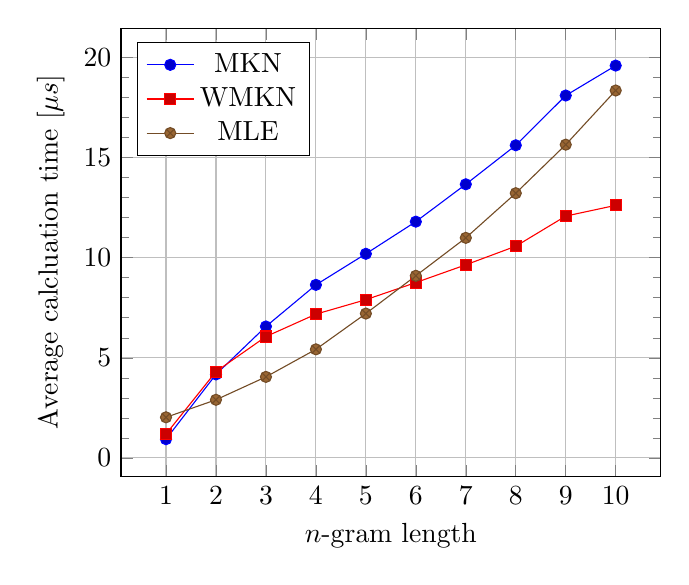
\begin{tikzpicture}[baseline]

\begin{axis}[
  xlabel = {$n$-gram length},
  xtick = {1, ..., 10},
  ylabel = {Average calcluation time [${\mu}s$]},
  minor y tick num = 4,
  grid = major,
  legend entries = {{MKN}, {WMKN}, {MLE}},
  legend pos = north west,
]

% MKN
\addplot table {
  n   us
  % sampled at N = 1000
  1    0.936
  2    4.171
  3    6.565
  4    8.643
  5   10.194
  6   11.800
  7   13.666
  8   15.614
  9   18.099
  10  19.594
};

% WMKN
\addplot table {
  n   us
  % sampled at N = 1000
  1    1.192
  2    4.311
  3    6.060
  4    7.180
  5    7.902
  6    8.758
  7    9.644
  8   10.573
  9   12.078
  10  12.614
};

% MKN
\addplot table {
  n   us
  % sampled at N = 1000
  1    2.028
  2    2.903
  3    4.047
  4    5.423
  5    7.210
  6    9.096
  7   10.991
  8   13.221
  9   15.645
  10  18.350
};

\end{axis}

\end{tikzpicture}
\end{document}

  \caption{\todo[inline]{TimeMKN-Caption}}
\end{figure}

\begin{figure}
  \centering
  \documentclass{standalone}
\usepackage[dvipsnames,svgnames,x11names]{xcolor}
\usepackage{tikz}
\usepackage{pgfplots}
\pgfplotsset{compat = 1.12}
\usepackage{../thesismath}
\begin{document}
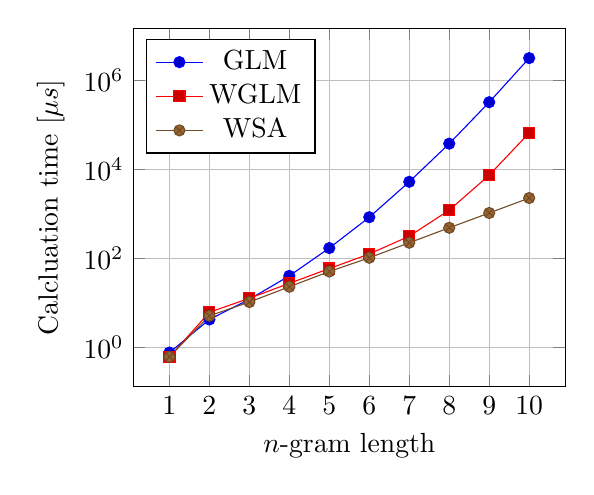
\begin{tikzpicture}[baseline]

\begin{axis}[
  xlabel = {$n$-gram length},
  xtick = {1, ..., 10},
  ylabel = {Calcluation time [${\mu}s$]},
  ymode = log,
  %yticklabel pos = right,
  minor y tick num = 4,
  grid = major,
  legend entries = {{GLM}, {WGLM}, {WSA}},
  legend pos = north west,
  scale = 0.8,
]

% GLM
\addplot table {
  n   us
  % sampled at N = 1000
  1   0.776
  2   4.296
  3   12.188
  4   40.981
  5   172.271
  % sampled at N = 100
  6   848.550
  7   5297.308
  % sampled at N = 10
  8   38045.228
  9   323947.490
  % sampled at N = 1
  10  3168612.887
};

% WGLM
\addplot table {
  n   us
  % sampled at N = 1000
  1   0.618
  2   6.223
  3   12.855
  4   27.786
  5   59.746
  % sampled at N = 100
  6   126.934
  7   317.936
  8   1223.680
  9   7463.531
  10  66226.605
};

% WSA
\addplot table {
  n   us
  % sampled at N = 1000
  1   0.624
  2   5.200
  3   10.572
  4   23.295
  5   51.307
  % sampled at N = 100
  6   104.217
  7   226.905
  8   491.327
  9   1056.845
  10  2287.351
};

\end{axis}

\end{tikzpicture}
\end{document}

  \caption{\todo[inline]{TimeGLM-Caption}}
\end{figure}

\chapter{Conclusion}


% Backmatter ===================================================================

\printbibliography

\begin{appendices}
  \chapter{Example Language Model Expansion}
\label{app:expansion}

Examples for \cref{ch:weightedsum}.

\section{Modified-Kneser-Ney}

\newcommand{\ProbMKNcab}[1]
  {\frac{\DiscountedCount(\text{a b c}) + \gamma(\text{a b}) #1}{\Count(\text{a b \Skp})}}
\newcommand{\ProbMKNcb}[1]
  {\frac{\DiscountedCount*(\text{\WSkp b c}) + \gamma(\text{b}) #1}{\ContCountIp(\text{\WSkp b \WSkp})}}
\newcommand{\ProbMKNc}
  {\frac{\ContCountIp(\text{\WSkp c})}{\ContCountIp(\text{\WSkp \WSkp})}}

Sample expansion for $\ProbMKN{\text{c}}{\text{a b}}$, assuming the sequence
``$\text{a b c}$'' was seen:
\begin{align}
  \ProbMKN {\text{c}}{\text{a b}} &= \ProbMKNcab{\ProbMKN*{\text{c}}{\text{b}}} \\
  \ProbMKN*{\text{c}}{\text{b}}   &= \ProbMKNcb{\ProbMKN*{\text{c}}} \\
  \ProbMKN*{\text{c}}             &= \ProbMKNc
\end{align}

Together:
\begin{equation}
  \ProbMKN {\text{c}}{\text{a b}} = \ProbMKNcab{\ProbMKNcb{\ProbMKNc}}
\end{equation}

By using the distributive property:
\begin{align}
  \ProbGLM {\text{c}}{\text{a b}} = {}
    & & \DiscountedCount (\text{a b c})     & \cdot\ \frac{1}{\Count(\text{a b \Skp})} \\
    &+& \DiscountedCount*(\text{\WSkp b c}) & \cdot\ \frac{\gamma(\text{a b})}{\Count(\text{a b \Skp}) \ContCountIp(\text{\WSkp b \WSkp})} \nonumber \\
    &+& \ContCountIp(\text{\WSkp c})        & \cdot\ \frac{\gamma(\text{a b}) \gamma(\text{b})}{\Count(\text{a b \Skp}) \ContCountIp(\text{\WSkp b \WSkp}) \ContCountIp(\text{\WSkp \WSkp})} \nonumber
\end{align}

\clearpage
\section{Generalized Language Model}

\newcommand{\ProbGLMcab}[2]
  {\frac{\DiscountedCount(\text{a b c}) + \frac{\gamma(\text{a b})}{2}\left(#1 + #2\right)}{\Count(\text{a b \Skp})}}
\newcommand{\ProbGLMcsb}[1]
  {\frac{\DiscountedCount*(\text{\WSkp \Skp b c}) + \frac{\gamma(\text{\Skp b})}{1} #1}{\ContCountIp(\text{\WSkp \Skp b \WSkp})}}
\newcommand{\ProbGLMcas}[1]
  {\frac{\DiscountedCount*(\text{\WSkp a \Skp c}) + \frac{\gamma(\text{a \Skp})}{1} #1}{\ContCountIp(\text{\WSkp a \Skp \WSkp})}}
\newcommand{\ProbGLMcss}
  {\frac{\ContCountIp(\text{\WSkp \Skp \Skp c})}{\ContCountIp(\text{\WSkp \Skp \Skp \WSkp})}}

Sample expansion for $\ProbGLM{\text{c}}{\text{a b}}$, assuming the sequence
``$\text{\text{a b c}}$'' was seen:
\begin{align}
  \ProbGLM {\text{c}}{\text{a b}}       &= \ProbGLMcab{\ProbGLM*{\text{c}}{\text{\Skp b}}}{\ProbGLM*{\text{c}}{\text{a \Skp}}} \\ \ProbGLM*{\text{c}}{\text{\Skp b}}    &= \ProbGLMcsb{\ProbGLM*{\text{c}}{\text{\Skp \Skp}}} \\
  \ProbGLM*{\text{c}}{\text{a \Skp}}    &= \ProbGLMcas{\ProbGLM*{\text{c}}{\text{\Skp \Skp}}} \\
  \ProbGLM*{\text{c}}{\text{\Skp \Skp}} &= \ProbGLMcss
\end{align}

Together:
\begin{align}
  &\ProbGLM{\text{c}}{\text{a b}} =\\
  &\qquad \ProbGLMcab{\ProbGLMcsb{\ProbGLMcss}}
                     {\ProbGLMcas{\ProbGLMcss}} \nonumber
\end{align}

By using the distributive property:
\begin{align}
  \ProbGLM {\text{c}}{\text{a b}} =
    & & \DiscountedCount (\text{a b c})          &             \cdot\  \frac{1}{\Count(\text{a b \Skp})} \\
    &+& \DiscountedCount*(\text{\WSkp \Skp b c}) &             \cdot\  \frac{\gamma(\text{a b})}{2 \Count(\text{a b \Skp}) \ContCountIp(\text{\WSkp \Skp b \WSkp})} \nonumber \\
    &+& \DiscountedCount*(\text{\WSkp a \Skp c}) &             \cdot\  \frac{\gamma(\text{a b})}{2 \Count(\text{a b \Skp}) \ContCountIp(\text{\WSkp a \Skp \WSkp})} \nonumber \\
    &+& \ContCountIp(\text{\WSkp\Skp \Skp c})    &             \cdot\  \frac{\gamma(\text{a b})}{2 \cdot 1 \Count(\text{a b \Skp})} \Big(  \frac{\gamma(\text{\Skp b})}{\ContCountIp(\text{\WSkp \Skp b \WSkp}) \ContCountIp(\text{\WSkp \Skp \Skp \WSkp})} \: + \nonumber \\
    & &                                          & \phantom{{} \cdot\  \frac{\gamma(\text{a b})}{2 \cdot 1 \Count(\text{a b \Skp})} \Big(} \frac{\gamma(\text{a \Skp})}{\ContCountIp(\text{\WSkp a \Skp \WSkp}) \ContCountIp(\text{\WSkp \Skp \Skp \WSkp})} \ \Big) \nonumber
\end{align}

  \chapter{SQL-Example}
\label{app:sql-example}

\todo[inline]{With database examples, and fully expanded SQL code, probably MKN query.}

  \chapter{Timeline}

\begin{itemize}
  \item Write chapters
    \begin{itemize}
      \item Introduction \textbf{<done>}
      \item Review of Considered language Models \textbf{<done>}
      \item Formulating Language Models as Weighted Sums \textbf{<done>}
      \item Fast Prefix Queries using Top-\emph{k} Joins (1-2day)
      \item Evaluation (3-4 days)
      \item Conclusion (1-2 days)
    \end{itemize}
  \item Run experiments \textbf{<almost done>}
  \item Finishing (3-4 days)
    \begin{itemize}
      \item Fix latex
      \item Reformulate shitty sentences
      \item Check formatting
    \end{itemize}
  \item Peer review, spelling correction (1-2 weeks)
  \item Make slides, prepare presentation \textbf{<almost done>}
\end{itemize}

\end{appendices}

\listoftodos

\end{document}
